


% Note that keywords are not normally used for peerreview papers.
%\begin{IEEEkeywords}
%IEEE, IEEEtran, journal, \LaTeX, paper, template.
%\end{IEEEkeywords}






% For peer review papers, you can put extra information on the cover
% page as needed:
% \ifCLASSOPTIONpeerreview
% \begin{center} \bfseries EDICS Category: 3-BBND \end{center}
% \fi
%
% For peerreview papers, this IEEEtran command inserts a page break and
% creates the second title. It will be ignored for other modes.




\chapter{Decentralized Architecture for Air Traffic Management in Urban Air Mobility}

\section{Urban air mobility setting}
Recent years have seen increased urbanization, economic expansion, underinvestment in infrastructure, and the rise of ride hailing services and e-commerce.  These changes have led to an increase in transportation delays, vehicle congestion during peak times, and environmental impacts resulting in escalating mobility challenges in urban areas which can negatively impact productivity~\cite{harriet2013assessment}. As population and congestion increase in these urban and suburban areas, mobility challenges are only expected to intensify. The emerging Urban Air Mobility (UAM) aviation market is being catalyzed by advances in increasingly autonomous systems, electric propulsion, and novel business models such as on-demand, aerial ride sharing, thereby helping to address congestion issues in urban areas~\cite{flightplan2030}.  

UAM has the potential to be a safe, functional solution to the air transportation problem for passengers and cargo in and around a densely populated urban area.  An air traffic management system that governs a large number of these novel UAM operations over a small geographical area in a safe and efficient fashion is key to the realization and deployment of the UAM vision.  The notion of on-demand, (near) point-to-point mobility that transits people or goods over congested urban areas offers the potential for reduced transit times, as well as decreased environmental impact, for low-noise, electrified UAM vehicles.  

UAM can not only help cities from an economic standpoint by allowing for faster movement of goods and people, but also has the potential to add to the public good by allowing for expedited public health services like air ambulances. However, establishing a framework, which allows for safe, orderly, and efficient flights in what will be a complex, high-traffic environment with competing requirements and priorities, remains crucial for UAM to be practically realized. 

In this chapter, we propose a method for scalable air traffic management (ATM) for UAM with \emph{provable guarantees} of safety properties. 


\subsection{Scalable and verifiable safety for UAM}

UAM presents challenges that cannot yet be handled in existing ATM approaches. Current and next generation ATM services, as described in~\cite{cook2007european,swenson2006next}, are designed to manage scheduled flights between established airports located in or near cities separated by a significant distance and occurring at conventional flight altitudes (e.g., above 10 000 ft). UAM will require management for on-demand, high-volume, short-range flights in close proximity to urban airspace (e.g., below 10 000 ft) with increasingly autonomous aircraft. Since these vehicles will be operating in urban airspaces with high traffic densities, they need to be able to operate with smaller separation standards than current ATM services can accommodate (e.g., closely spaced altitude separation). Any traffic management system for UAM will also need to be able to handle unpredictable situations in a safe manner without overly compromising the performance of the entire system. 

Furthermore, the scale and density of projected UAM operations will far exceed the safe workload capacity of human controllers, necessitating the deployment of increasingly autonomous solutions for functions like aircraft management (e.g., managing flightpath and altitude requests, managing airborne and ground based holding times, etc.) and aircraft separation. Currently, there is no established infrastructure for air traffic management of a scalable UAM concept of operations.  A traffic management system for small unmanned aerial systems (UAS) called UTM (UAS Traffic Management) has been proposed, and takes a federated approach to ensuring airspace access~\cite{PRKRJJ2016}.  This approach may enable the incorporation of multiple safety oriented services~\cite{MBYDLGMC2018} such as aircraft separation~\cite{Daidalus} and geo-fencing~\cite{NCDDASC2018}.  However, UTM is designed primarily for small cargo carrying air vehicles. As such, UTM is not capable of providing the safety guarantees that a system involving larger passenger carrying vehicles would require. 

More crucially, there are concerns with respect to scalability. Under current aviation paradigms, air traffic management is carried out in a centralized fashion by air traffic controllers.  The U.S. National Airspace System (NAS) is comprised of 5.3 million square miles of domestic airspace and 24 million square miles of oceanic airspace.  There are approximately 5,000 flights airborne at any given moment.  Over 14,000 air traffic controllers manage these aircraft and perform multiple safety-critical functions, such as air traffic separation which guarantees that a minimum spacing between aircraft is maintained \cite{FAAData}.  In contrast, for UAM operations to deploy at scale for profit, it will be necessary to have hundreds (or even thousands) of UAM aircraft aloft over an urban airspace under 500 square miles~\cite{goyal2018urban}.  The sheer number of vehicles, along with the necessary reduced separation criteria between them in order to achieve the required densities, will require the development of increasingly autonomous capabilities for aircraft clearance, separation, and flow management in the UAM ecosystem.  

Deploying increasingly autonomous systems in the US airspace is a challenge. Commercial aviation is among one of the most safety-critical systems in the world and has stringent standards for the design, deployment, and operation of aircraft and air traffic control systems. These regulations are detailed in chapter 14 of the Code of Federal Regulations (14 CFR). The ability to assure increasingly autonomous systems to aviation grade standards is thus crucial for their acceptance.  Safety-critical functions such as aircraft separation must provide strict guarantees on their behavior and the correctness of their outcomes.  Thus, increasingly autonomous air traffic management systems will have to tackle the dual issues of scalability and verifiable safety in order to be deployed in the NAS. There is a therefore, a pressing need to explore the design of an ATM system architecture capable of safely and efficiently managing UAM operations. 

\subsection{Challenges in air traffic management for UAM}

Guaranteeing global satisfaction of safety properties for UAM operations has the following key challenges

\begin{itemize}
    \item The setting encompasses multiple service providers and stakeholders, each with potentially competing priorities and requirements. Consequently, the full state of the entire fleet of vehicles is unlikely to be controlled or even observed by a single entity. 
    \item UAM will operate in a complex and diverse airspace environment(e.g., Class G \cite{FAA2014}, Class B etc.) that must support both conventional operations using legacy aircraft as well as emerging operations. Therefore verifying safety of such an evolving system at design-time is not practical.
    \item While a centralized solution process allows for easier verification of correctness, the resulting state space explosion entailed in synthesis, especially under the projected traffic demands, makes a centralized solution computationally untenable. 
\end{itemize}


Removing reliance on full state-information for control requires a version of distributed synthesis. However, except for a few restricted classes of architectures, the distributed synthesis problem is undecidable~\cite{SCHEWE2014203}. The decidable versions of the problem lack practical solutions due to their non-elementary complexity~\cite{Schewe08}. Significant effort in runtime monitoring in this area is focused on providing efficient solutions by exploiting  the structure of the system~\cite{FalconeJNBB15,CassarF16} or the specification~\cite{FrancalanzaS15,BauerF16}.  We employ this idea by constructing an architecture with a hierarchical decomposition of the UAM operations space motivated by the physical and geographical infrastructure required to field the system. We then design a framework for synthesis in this architecture with provable guarantees of correctness. Our framework has the following properties:


\begin{itemize}
	\item \emph{Scalability} - UAM operations are envisioned to occur at a scale well beyond the capabilities of current air traffic management approaches, as current day approaches are typically labor-intensive. It is crucial to safely guarantee operations of increasingly autonomous vehicles at scale in order for UAM to be commercially viable. 
	
	\item \emph{Decentralization} - The environment is likely to encompass multiple service providers and stakeholders. Each stakeholder will have potentially competing priorities and requirements. Consequently, the full state of the entire system is unlikely to be controlled or even observed by a single entity.
	
	\item \emph{Transparency} - With companies ranging from startups to corporations developing UAM vehicles, services, and capabilities, there is a disconnect between regulation and the pace of technological development. Bridging the gap between regulation and real-world implementation practices is necessary for a viable path to deployment. 
	
	\item \emph{Flexibility} - The technological and regulatory landscape of UAM is rapidly changing. Any proposed framework that cannot efficiently incorporate a change in regulation or emerging capabilities is not a viable solution. 
	
	\item \emph{Auditability} - All violations of regulations must be formally accounted for and reported. Our proposed method implicitly allows for such an analysis, as it not only synthesizes a control strategy for air traffic management but also the associated violation. 
\end{itemize}

\subsection{UAM ATM architecture}
We propose a decentralized, hierarchical UAM ATM architecture for provably correct operations. We divide up the responsibilities of an ATM architecture for UAM into two broad classes
\begin{itemize}
    \item[1.] Pre-flight authorization: receiving flight requests with little notice, identifying a safe route, and authorizing the departure.
\item[2.] Dynamic airspace management: managing routes and in-flight aircraft in response to an unpredictable environment stemming from the on-demand trip scheduling.
\end{itemize}

Both of these responsibilities are complex and safety critical, due to the lack of schedules, projected high traffic densities and diverse nature of the vehicles and operations sharing the airspace (e.g., UAS, general aviation aircraft etc.). Pre-departure planning and de-conflicting flight routes before take-off have been studied extensively in the literature \cite{6011668,7415976,7934784}. More recently, there have been efforts in applying these works in an on-demand UAM setting \cite{guerreiro2019mission}. Here, we primarily focus on the latter case of guaranteeing safety during dynamic flight operations and will assume the existence of an assured scheduler that is able to give pre-flight authorization for routes given passenger requests. 

In our proposed UAM ATM architecture, we leverage the geographical location of infrastructure to divide the region into sectors that are each overseen by \emph{vertihubs}. UAM vehicles take off and land from a landing pad, called a vertipad, which includes the final approach and takeoff (FATO) area. A vertiport is comprised of several vertipads, the respective vertipad FATOs, and charging and maintenance facilities.  A vertihub is comprised of several vertiports.  Vertihubs provide air traffic control services (i.e., real time control of aircraft movement) between vertiports under their control and air traffic management services (i.e., strategic and long term planning of aircraft movement and flows) for vehicles transiting between adjacent vertihubs.  Figure~\ref{fig:uam_architecture} provides a visual representation of vertiports and vertihubs.  Such an architecture is similar to how airspace in the Terminal Radar Approach Control is managed, but is more general in its approach to tackling balkanization. 


\begin{figure}
	\centering
	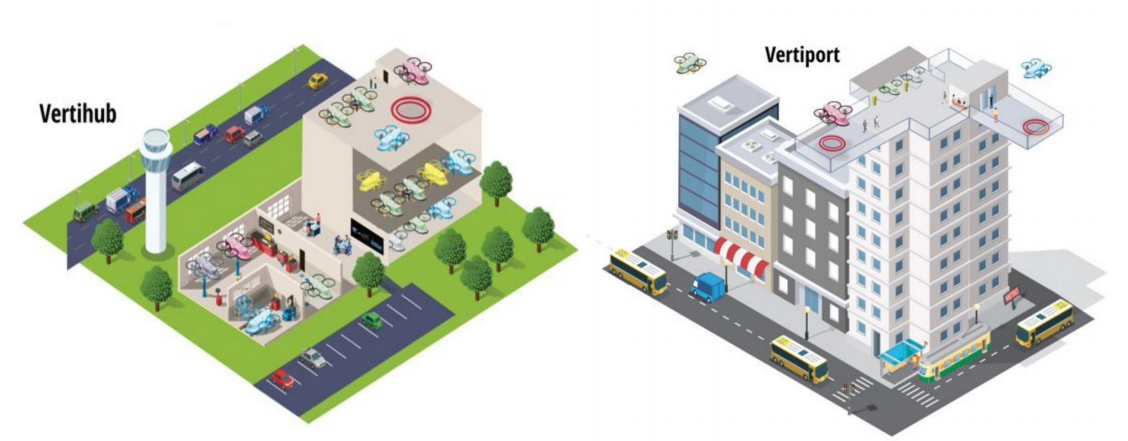
\includegraphics[width=0.98\columnwidth]{UAM-NFM/Figures/vert.PNG}
	\caption{Vertihub and vertiport depiction}
	\label{fig:uam_architecture}
\end{figure}


The UAM setting is unique as most flights will be on-demand and hence will require a controller that can \emph{react} to an unpredictable environment and provide guarantees of safety and liveness. Reactive synthesis~\cite{bloem2018graph} is a natural candidate to produce such controllers. A user (such as a regulatory body) can specify specifications in linear temporal logic for the operations of each vertihub and vertiport in the system. The task is to synthesize controllers for each vertihub and vertiport separately, guaranteeing that, together, the joint operation of the global system satisfies the conjunction of all specifications while still guaranteeing progress for the vehicles. In order to ensure that each controller does not impede the ability of other controllers to satisfy their requirements, we introduce a contract-based synthesis method which we formulate as a Generalized Reactivity(1) (GR(1))~\cite{bloem2012} synthesis problem that can be solved efficiently~\cite{wolff2013efficient,alur2016compositional}. Hence, our proposed solution architecture is scalable without sacrificing any safety or liveness guarantees. 


\subsection{Contributions}
This work is the first that considers a hierarchical, decentralized synthesis framework for UAM air traffic management. We use temporal logic for a formal representation of safety regulations and provably verify that these properties are satisfied across the global system. The contributions are as follows:

\begin{itemize}
	\item We design an architecture that allows a user (such as a regulatory body interested in guaranteeing safe operations) to specify safety requirements for the operations at each vertihub and vertiport. 
	\item The architecture allows the controller for each vertihub and vertiport to be synthesized separately, hence avoiding the state-space explosion of centralized synthesis. 
	\item We use contracts to guarantee that the joint interactions of all the individual controllers still satisfy all the safety requirements, and that vehicles will still make progress towards their goals. 
	\item We provide high-fidelity simulations on large-volume projected UAM traffic data to showcase the applicability of our proposed architecture.
\end{itemize}

\subsection{Path to deployment}

Assessing the safety of an increasingly autonomous system relies on being able to bound the behavior and interactions of the components of the system as well as its interfaces with its operational environment. Performance-based regulation is employed in aviation to specify explicit properties that must be evinced by a component or element of the system (and/or operational environment) in order for the system safety claims to be met.  For example, 14 CFR \S 107.49 (d) states that: “If the small unmanned aircraft is powered, ensure that there is enough available power for the small unmanned aircraft system to operate for the intended operational time”.  This fuel requirement forms a temporal logic constraint on the vehicle during its flight. The controller synthesis method for the vertihubs must adhere to this constraint, in order to demonstrate compliance to 14 CFR \S 107.49.  The minimum violation guarantees provided by the presented synthesis process help to demonstrate that this regulation will be satisfied as much as possible throughout the flight process.  Thus, the guarantees provided by the synthesis method presented in this chapter may serve as a partial means of compliance to the regulation---supplemented with the generation of test and design analysis artifacts as well as operational procedures.

The presented synthesis framework provides a path to deployment of these increasingly autonomous systems in safety-critical contexts.  Air traffic management services, such as aircraft separation, may then be offered in a UAS Traffic Management (UTM) inspired framework, which interfaces with today’s traditional Air Traffic Management framework~\cite{PRKRJJ2016}. In this framework,  authority may be delegated by the FAA to provide select air traffic management services such as low-altitude weather information, congestion management, terrain avoidance, route planning, re-rerouting, separation management, and contingency management~\cite{MBYDLGMC2018,NCDDASC2018}.  One of the main attributes of the UTM system is that it does not require human operators to monitor every vehicle continuously, as in the traditional ATM system, thereby enabling increasingly autonomous realizations of specified air traffic management functions.  NASA has led UTM research over the past five years, and is currently involved in the development and testing of a prototype UTM system with the FAA, in conjunction with numerous industry and public agency partners.  

I believe that integration of the approach in this chapter into a UTM-like construct provides a path to deployment for UAM operations, as the provided safety guarantees will greatly enhance the assurance case for higher-risk operations currently not supported by UTM (e.g., operations in dense urban environments with UAS exceeding 55 lbs).


\section{Related work}

 Some preliminary work is being done in cooperative ATM for next generation air traffic management \cite{prevot2005co}, but this work considers a scheduled approach for large passenger aircraft and cannot handle management for on-demand flights. Similarly, work has been done on distributed control for ATM of small unmanned aerial systems (UAS) \cite{FSLLK2015}, but this work relies on cloud based architectures that do not currently satisfy strict aviation safety requirements.  Hybrid control approaches have been applied \cite{tomlin1996hybrid}, however scalability proves to be an issue.


To the best of our knowledge, this is the first approach to
controller synthesis with safety guarantees for large-scale UAM ATM operations. Formally verified tools such as DAIDALUS~\cite{Daidalus} provide safety guarantees at lower levels of operations, however, they do not handle the fleet-level operations. The most similar approach to the one presented in this chapter is \emph{runtime enforcement}~\cite{Falcone10,Schneider00} of a specified property, in which a synthesized module detects and alters the behavior of the system in a way that maintains the desired property. An existing approach called shielding~\cite{BloemKKW15,KonighoferABHKT17} uses reactive synthesis and assumes that the shield has full knowledge and control of the whole system --- in this case the entire UAM system and the vehicles it handles. 

A technique for synthesizing quantitative shields for multi-agent systems in a fully centralized manner was presented in \cite{multiagentshield}. All these approaches rely on restrictive assumptions on runtime communication (i.e., full network coverage) and the extent of awareness and control authority of the shield (e.g., the shield can affect any agent in the network instantaneously). This requirement was relaxed in~\cite{bhnfm} where a local shield was synthesized for each sector with contracts between neighbors to guarantee global correctness. However, the approach was formulated only for specific safety properties (e.g., minimum-separation) and not more general properties such as liveness as is done here. We do not consider quantitative properties or optimality of behavior in this work, as the primary focus is the guarantee of specifications.

The work detailed in the following directly extends~\cite{bhnfm} by generalizing the class of allowable safety properties to any property in the GR(1)~\cite{bloem2012} fragment of linear temporal logic. Furthermore, the work in~\cite{bhnfm} was limited to very specific vehicle behaviors, and could not handle take-off or landing requests. In this work, we introduce vertiport controllers that operate in the sector regions to additionally handle take-off and landing requests. The induced hierarchical structure allows for \emph{separation of concerns} between the vertihub and vertiport controllers. A decentralized, hierarchical approach for ATM was proposed in~\cite{6011668}, but unlike the setting in this chapter, cannot handle temporal logic specifications. Hence, we are able to systematically synthesize controllers for ATM that can guarantee complex temporal requirements unlike conventional ATM approaches such as~\cite{6011668}. 


\section {Problem setting}
%\subsection{Overview}\label{sec:problemoverview}
 Consider an environment consisting of an operating space and a network formed from a series of $k$ UAM vertiport hubs labeled $V_1,\cdots,V_k$. A UAM vertiport hub (henceforth referred to as a vertihub) consists of a grouping of multiple vertiports, each of which may have multiple takeoff/landing pads. A vertihub is responsible for managing requests by UAM vehicles (henceforth referred to as vehicles) to either \emph{land at} or \emph{take off from} a desired vertiport in its region or \emph{pass through} to a neighboring region. Each vertiport inside a vertihub is in charge of taking off and landing vehicles at its landing pads. An example of such an environment is illustrated in Figure~\ref{fig:RegionsOutline}. Note that vertihub control regions need not be circular. 
\begin{example}
The vertihub controller for region $V_6$ in Figure~\ref{fig:RegionsOutline} controls the operational area defined by $V_6 - (V_6 \cap V_5)$. The area of overlap $H_{56} = V_5 \cap V_6$ is the region where the handoff takes place, wherein the vertihub controller of the region the vehicle is about to enter takes responsibility for the vehicle.
Hence, $V_6$ can force vehicles incoming from $V_5$ to loiter in the handoff region $H_{56}$ until it is safe to allow them to enter.
\end{example}

The number of vehicles allowed inside each vertihub is upper bounded both by the separation standards between the vehicles as well as with the complexity of the airspace (e.g., intersection with general aviation traffic etc.).
Vertihubs cannot accept vehicles (i.e., accept a handoff) if the additional vehicle exceeds the maximum operational capacity or induces a conflict. Furthermore, vertiports cannot allow vehicles to take-off if it will violate the maximum operational capacity of the vertihub, and must force incoming vehicles to loiter if all of their pads are occupied. In order to avoid violating airspace requirements and to avoid build up of loitering vehicles (which can delay vehicles desiring to pass through or create safety issues), a vertiport must coordinate with its corresponding vertihub. We model the vertihub controller and vertiport controllers as \emph{reactive systems}.
%The hub can then act tactically by blocking a vehicle's entry to the region by making it loiter in a \emph{handoff region}.

\paragraph*{\textbf{Definition}}
We consider a finite set $\inp$ ($\out$) of Boolean \emph{inputs (outputs)}.
The input alphabet is
$\ialphabet=2^\inp$, the output alphabet is $\oalphabet=2^O$, and
$\alphabet=\ialphabet \times \oalphabet$. The set of finite (infinite) traces
over $\alphabet$ is denoted by $\alphabet^*$ ($\alphabet^\omega$), and
we define $\alphabet^{\infty} = \alphabet^* \cup \alphabet^\omega$.  A reactive system is a
tuple $\design = (\states,q_{0},\ialphabet,\oalphabet,\delta,\lambda)$,
where
$\states$ is a finite set of states,
$q_{0} \in \states$ is the initial state,
$\ialphabet$ is the input alphabet,
$\oalphabet$ is the output alphabet,
$\delta: \states \times \Sigma_{\inp} \to \states$ is the complete transition function, and $\lambda : \states \times \Sigma_{\inp} \to \Sigma_{\out}$ is the output function.
%
Given an input trace $\itrace = x_0 x_1 \ldots \in \ialphabet^\infty$, a reactive system $\mathcal{\design}$ produces an
output trace $\otrace = \mathcal{\design}(\itrace) = \lambda(q_0, x_0)
\lambda(q_1, x_1) \ldots \in \oalphabet^\infty$ with $q_{i+1} = \delta(q_i, x_i)$ for all $i \ge 0$.
The set of words produced by
$\mathcal{\design}$ is denoted $\lang(\mathcal{\design}) = \{\itrace \parallel \otrace \in
\alphabet^\infty \mid \mathcal{\design}(\itrace) = \otrace\}$.



\begin{figure}[h!]
	\centering

\newcommand{\OperatorSpace}[5]{
				%\draw[rounded corners = 15pt,dashed] (#1-#4,#2-#5) rectangle (#1+#4,#2+#5);
		\fill[fill=green,opacity=0.2] (#1,#2) circle (#3);
		\draw[draw = black,dashed](#1,#2) circle (#3);
		%\node at (#1,#2-#5+0.5) {$V_{#6}$};
	}

	

		\subfloat[ Example UAM operating environment \label{fig:RegionsOutline}]{
		\scalebox{1.75}{
		\begin{tikzpicture}[scale=0.3]
			\OperatorSpace{0}{0}{3}{5}{5}
			%\node at (-4.25,4.25){$S_1$};
			\node at (-1.5,1.5){$V_1$};
			\OperatorSpace{3}{-4}{3}{5}{5}
			%\node at (-1.25,-8.25){$S_2$};
			\node at (2.5,-4.5){$V_2$};
			\node[red] at (2.5,3) (H13) {$H_{13}$};
			\draw [->,red,line width = 0.75mm] (H13) -- (2.5,1.25);
			\OperatorSpace{5}{0}{3}{5}{6}
			%\node at (5-4.25,5.5){$S_3$};
			\node at (5-0.5,2){$V_3$};
			\node[red] at (6.5,3.5) (H35) {$H_{35}$};
			\draw [->,red,line width = 0.75mm] (H35) -- (6.75,0.65);
			\OperatorSpace{10}{0}{4}{6}{7}
			
			\node at (8.5-0.5,-5.5){$V_4$};
% 			\node[red] at (6.5,3.5) (H35) {$H_{35}$};
			\draw [->,red,line width = 0.75mm] (H35) -- (6.75,0.65);
			\OperatorSpace{6.5}{-4}{2.5}{0}{0}
			
			%\node at (10+5.25,-6.5){$S_5$};
			\node at (10+1.5,-1.5){$V_5$};
			\OperatorSpace{15}{2}{3}{5}{5}
			\fill[blue] (-1.5,-1.5) rectangle (-1,-1);
			%\node at (15-4.25,5+3.25){$S_6$};
			\node at (15,3.5){$V_6$};
			\node[red] at (11,4.5) (H56) {$H_{56}$};
			\draw [->,red,line width = 0.75mm] (H56) -- (12.5,2.75);
			\draw (17,3) node[cross,blue]{};
			\draw[blue,line width = 0.5mm] plot [smooth,tension=1] coordinates{(-1.5,-1.5) (3,0.5) (10,0) (17,3)};
			\draw (-0.5,2) node[cross,black]{};
			\fill[black] (7.5,-5.5) rectangle (7.0,-5.0);
			\draw[black,line width = 0.5mm] plot [smooth,tension=1] coordinates{(-0.5,2) (3,-0.5) (7,-5.0)};
			
		\end{tikzpicture}}}\\
\subfloat[Connectivity graph \label{fig:Environment_directed}]{
\scalebox{1.25}{
\begin{tikzpicture}[auto,node distance=8mm,>=latex,font=\small]
        \tikzstyle{round} = [thick,draw=black,circle]
\tikzstyle{action} = [circle, draw, fill=black,inner sep=0pt, minimum size=4pt]
\node[round] (s1) {$\design_{1}$};
\node[round, right=15mm of s1] (s3){$\design_{3}$};
\node[round, below right=15mm and 5mm of s1] (s2){$\design_{2}$};
\node[round, right=15mm of s3] (s5){$\design_{5}$};
\node[round, right=10mm of s2] (s4){$\design_{4}$};
\node[round, right= 10mm of s5] (s6){$\design_{6}$};

\draw[<->] (s1) -- node[left]{$e_{12}$} (s2);
\path[<->,draw] (s1) -- node{$e_{13}$} (s3);
\path[<->,draw] (s2) -- node{$e_{23}$} (s3);
\path[<->,draw] (s2) -- node{$e_{24}$} (s4);
\path[<->,draw] (s3) -- node{$e_{34}$} (s4);
\path[<->,draw] (s3) -- node{$e_{35}$} (s5);
\path[<->,draw] (s4) -- node[right]{$e_{45}$} (s5);
\path[<->,draw] (s5) -- node[below]{$e_{56}$} (s6);

% \path[->,draw] (s1) edge[loop above] node {$e_{1}$} (s1);
% \path[->,draw] (s2) edge[loop below] node {$e_{2}$} (s2);
% \path[->,draw] (s3) edge[loop above] node {$e_{3}$} (s3);
% \path[->,draw] (s4) edge[loop below] node {$e_{4}$} (s4);
% \path[->,draw] (s5) edge[loop above] node {$e_{5}$} (s5);
% \path[->,draw] (s6) edge[loop above] node {$e_{6}$} (s6);

\end{tikzpicture}}}

\caption{
(a) Green circles correspond to the region of a vertihub. UAM vehicles (blue and black) move between origin-destination vertiports in the environment.
(b)
The corresponding connectivity graph $G_\design$ of the vertihub controllers $\design$ modeling the sectors $V$. 
Each edge $e_{ij}$ corresponds to $\design_i$ and  $\design_j$ being connected, i.e., the outputs of $\design_i$ are inputs to $\design_j$ and vice versa.
}
%		\setlength{\belowcaptionskip}{-2pt}
	       %\label{fig:RegionsOutline}
    \end{figure}

Ensuring the safety of the takeoff and landing operations at vertiports that share the same airspace must be balanced with bounding the delays experienced by vehicles. Furthermore, vehicles cannot loiter indefinitely due to energy constraints.
Hence, vertihubs must additionally guarantee a finite upper bound on the delays experienced by vehicles.
All of these requirement guarantees (and others) can be expressed as \emph{temporal logic specifications} that controllers must satisfy. %In addition to satisfying their own specification, each controller must not cause other controllers to violate their specification. We formalize this notion in Section~\ref{sec:distshield}. 


\paragraph*{\textbf{Definition}}
%
A \emph{linear temporal logic (LTL) specification} $\varphi$ defines a set of allowed traces $L(\varphi) \subseteq \plays(\design)$ for the reactive system $\design$.  A reactive system $\design$ is \emph{winning} with respect to specification $\varphi$ iff $L(\design) \subseteq L(\varphi)$ and is denoted $\design \models \varphi$. Given a set of propositions \texttt{AP}, a formula in LTL describes a language in $(2^{\texttt{AP}})^\omega$. LTL extends Boolean logic by the introduction of temporal operators such as $\bigcirc$ (next time), $\LTLglobally$ (always), $\LTLfinally$ (eventually), and $\mathcal{U}$ (until). 


 Informally, the main problem addressed in this paper is designing \emph{controllers} for vertihubs and vertiports that guarantee all safety and progress requirements, assuming they have been correctly captured in the design process. More formally, the task of computing a satisfying controller in reactive systems involves constructing the function $\lambda$ and can be typically framed as computing the \emph{winning strategy of a game}. 



\paragraph*{\textbf{Definition}}
%
A \emph{game structure} is a tuple 
$\game = (\states, \state_0, \alphabet, \delta,\Acc)$,
where 
\begin{itemize}
\item $\states$ is a finite set of states, $\state_0 \in \states$ the initial state,
\item $\alphabet = (\ialphabet \times \oalphabet)$ is the alphabet of actions available to the environment and the controller respectively, 
\item $\delta: \states \times \alphabet \rightarrow \states$
is a complete transition function, that maps each state, input (environment action) and output (controller action) to a successor state.
\item $\Acc: \left(\states \times \alphabet \times \states\right)^\omega \rightarrow \mathbb{B}$ is the \emph{winning condition} of the game. 
% \item $\mathcal L:\gstates
% \rightarrow \ialphabet \times \oalphabet$ is the labeling
% function.
\end{itemize}


At every state $\state \in \states$ (starting with
$\state_0$), the environment chooses an input $\isymb \in
\ialphabet$, and then the controller chooses some output $\osymb
\in \oalphabet$. These choices define the next state $\state' =
\delta(\state,(\isymb, \osymb))$, and the process then continues from $\state'$. This order of moves
ensures that at each step the controller's action reacts to the \emph{current}
action of the environment. The resulting
(infinite) sequence $\pi = (\state_0,\symb_{\inp,0},
\symb_{\out,0}, \state_1) (\state_1,\symb_{\inp,1},
\symb_{\out,1}, \state_2) \ldots$ is
called a \emph{play}, where $\state_0$ is the initial state, and for every $i \geq 0$ we have that $\state_{i+1} = \delta(\state_i,\symb_{\inp,i},\symb_{\out,i})$.  A play $\pi$ is \emph{winning} if $\Acc(\pi) = \top$. 
%The set $L(\game)$ is the set of all plays in the game $\game$.


We consider winning conditions expressed from a fragment of LTL specifications called \emph{Generalized Reactivity 1} (GR(1)), which is common in a variety of practical applications~\cite{Moarref18,Alonso18,bh18,Maoz2015}.
A GR(1) winning condition is defined by sets of states $S_\inp, S_\out \subseteq \states$, $E_i \subseteq \states$ for $i=1,\ldots,m$ and $F_j \subseteq \states$ for $j=1,\ldots,n$, and consists of all plays $ \pi$ such that if $\pi \in \LTLglobally S_\inp \cap \LTLglobally\,\LTLfinally\, E_{i}$ for all $i=1,\ldots,m$, then $\pi \in \LTLglobally S_\out \cap \LTLglobally\,\LTLfinally\, F_{j}$ for all $j=1,\ldots,n$. Intuitively, for a play $ \pi$ to be winning, whenever the environment satisfies the assumptions $\LTLglobally\, S_\inp,\LTLglobally\,\LTLfinally\, E_{1},\ldots,\LTLglobally\,\LTLfinally\, E_{m}$, then the controller must satisfy all the guarantees $\LTLglobally\, S_\out,\LTLglobally\,\LTLfinally\, F_{j},\ldots,\LTLglobally\,\LTLfinally\, F_{n}$. By abuse of logical operators, we abbreviate GR(1)  conditions as
$$\left(\LTLglobally\, S_\inp \wedge \bigwedge_{i=1}^{m}  \LTLglobally\,\LTLfinally\, E_{i}\right) \implies
\left(\LTLglobally\, S_\out \wedge \bigwedge_{j=1}^{n} \LTLglobally\,\LTLfinally\,F_{j}\right).$$


\paragraph*{\textbf{Definition}}
%
% We seek to compute a strategy for the agent to enforce a given winning condition, or determine that it cannot ensure winning.

A \emph{strategy for the controller} is a function $\rho_\out:
\prefs(\game) \times \ialphabet \rightarrow
\oalphabet$ which maps a prefix of a run (the history of the play so far) and an action of the environment to an action of the controller. 
A \emph{strategy for the environment} is a function $\rho_\inp: \prefs(\game)\rightarrow \ialphabet$ that maps the prefix of the play so far to an action of the environment. We denote the sets of all strategies for the controller and for the environment by $\mathcal{M}_\out $ and $\mathcal{M}_\inp$ respectively.

Every pair of strategies $\rho_\out \in \mathcal{M}_\out$ for the controller and $\rho_\inp \in \mathcal{M}_\inp$ for the environment define a play, denoted by $\Pi(\rho_\out,\rho_\inp)$. More precisely,  
$\Pi(\rho_\out,\rho_\inp) = \pi = (\state_0,\symb_{\inp,0},\symb_{\out,0}, \state_1) 
(\state_1,\symb_{\inp,1}, \symb_{\out,1}, \state_2) \ldots \in \plays(\game)$
where
for every $i \geq 0$, $\symb_{\inp,i} = \rho_\inp(\pi[0,i])$ and $\symb_{\out,i} = \rho_\out(\pi[0,i],\symb_{\inp,i})$.
Similarly, we define the set of plays starting at a state $g$ that are consistent with $\rho_\out$, denoted $\plays(\design,\rho_\out,g)$.

Given a game structure $\design$ and a winning condition $\varphi$ for the agent, the synthesis problem is to generate a strategy $\rho_\out\in \mathcal{M}_\out$ for the controller such that for every strategy $\rho_\inp \in \mathcal{M}_\inp$ for the environment it holds that $\Pi(\rho_\inp,\rho_\out) \in \varphi$, i.e., all resulting plays satisfy $\varphi$.
In such cases we say that \emph{$\rho_\out$ satisfies $\spec$}, denoted $\rho_\out\models\spec$.




% \subsection{Basic notations}
% We consider reactive systems with a finite set $\inp$ ($\out$) of Boolean \emph{inputs (outputs)}.
% The input alphabet is
% $\ialphabet=2^\inp$, the output alphabet is $\oalphabet=2^O$, and
% $\alphabet=\ialphabet \times \oalphabet$. The set of finite (infinite) traces
% over $\alphabet$ is denoted by $\alphabet^*$ ($\alphabet^\omega$), and
% we define $\alphabet^{\infty} = \alphabet^* \cup \alphabet^\omega$.  

% \subsection{Reactive systems}

% A \emph{reactive system} is defined by a
% tuple $\design = (\states,q_{0},\ialphabet,\oalphabet,\delta,\lambda)$,
% where
% $\states$ is a finite set of states,
% $q_{0} \in \states$ is the initial state,
% $\ialphabet$ is the input alphabet,
% $\oalphabet$ is the output alphabet,
% $\delta: \states \times \Sigma_{\inp} \to \states$ is the complete transition function, and $\lambda : \states \times \Sigma_{\inp} \to \Sigma_{\out}$ is the output function.
% %
% Given an input trace $\itrace = x_0 x_1 \ldots \in \ialphabet^\infty$, a reactive system $\mathcal{\design}$ produces an
% output trace $\otrace = \mathcal{\design}(\itrace) = \lambda(q_0, x_0)
% \lambda(q_1, x_1) \ldots \in \oalphabet^\infty$ with $q_{i+1} = \delta(q_i, x_i)$ for all $i \ge 0$.
% The set of words produced by
% $\mathcal{\design}$ is denoted $\lang(\mathcal{\design}) = \{\itrace \parallel \otrace \in
% \alphabet^\infty \mid \mathcal{\design}(\itrace) = \otrace\}$.
% In reactive systems, the synthesis task involves constructing the function $\lambda$ and can be typically framed as computing the \emph{winning strategy of a game}. 




% \subsection{Specifications}
% %
% A \emph{linear temporal logic (LTL) specification} $\varphi$ defines a set of allowed traces $L(\varphi) \subseteq \plays(\design)$ for the reactive system $\design$.  A reactive system $\design$ is \emph{winning} with respect to specification $\varphi$ iff $L(\design) \subseteq L(\varphi)$ and is denoted $\design \models \varphi$. Given a set of propositions \texttt{AP}, a formula in linear temporal logic (LTL) describes a language in $(2^{\texttt{AP}})^\omega$. LTL extends Boolean logic by the introduction of temporal operators such as $\bigcirc$ (next time), $\LTLglobally$ (always), $\LTLfinally$ (eventually), and $\mathcal{U}$ (until). 





%In the following, we make use of LTL operators $\LTLglobally$ and $\LTLfinally$ which are operators for \emph{always} and \emph{eventually} respectively. For full details on LTL syntax, we refer the reader to~\cite{MCBook}.

% A \emph{safety} winning condition $\varphi$ is defined by a set of states $S \subseteq G$ and is such that for a play $\overline{\pi}\in \plays(\game)$ we have $\overline\pi\in\varphi$ if and only if $g_i \in S$ for all $i \in\mathbb{N}$.

% A \emph{\buchi} winning condition $\varphi$ is defined by a set of states $F \subseteq G$ and is such that for a play $\overline{\pi} \in \plays(\game)$ we have $\overline\pi\in\varphi$ iff $\inf(\overline{\pi})\cap F \neq \emptyset$,  where $\inf(\overline{\pi}) \subseteq G$ is the set of states that occur infinitely often in $\overline{\pi}$.
% We abbreviate the \buchi condition as $\varphi = \LTLglobally\,\LTLfinally\, F$.



%Note that if the agent has a winning condition $\varphi$, then all plays in $\plays(\game)\setminus\varphi$ are winning for the environment player.




\iffalse
\subsection{Serial composition}
Consider two reactive systems  $\design = (\states,q_{0},\ialphabet,\oalphabet,\delta,\lambda)$ and $\shield = (\states', q_{0}',\alphabet', \delta',\lambda')$.
The \emph{serial composition} of $\design$ and $\shield$ is obtained by feeding the output of $\design$ to $\shield$ and results in a new reactive system $\design \comp \shield=(\hat{\states}, \hat{q_{0}}, \ialphabet,\oalphabet, \hat{\delta},
\hat{\lambda})$, where
   $\hat{\states} = \states \times \states'$,
   $\hat{q_{0}} = (q_{0}, q_{0}')$,
   $\hat{\delta}((q,q'),\isymb) = (\delta(q,\isymb), \delta'(q',(\isymb,\lambda(q,\isymb))))$, and
   $\hat{\lambda}((q,q'),\isymb) = \lambda'(q',(\isymb,\lambda(q, \isymb)))$.
\fi
   
% \subsubsection{Multi-agent reactive systems}
% A \emph{multi-agent reactive system} $\design$ is a tuple $(\proc, \ialphabet,  \oalphabet)$, where $\proc = \{\proc_1,\ldots,\proc_n\}$ is a set of agents, where each $\proc_i = (\states_i, q_{0,i},\ialphabeti,\oalphabeti,\delta_i,\lambda_i)$ is a reactive system. For more details on the construction of multi-agent reactive system, we refer the reader to \cite{multiagentshield}. 

%Since we perform a localized synthesis procedure in this paper, the multi-agent reactive systems dealt with in \cite{multiagentshield} will instead be decentralized single-agent reactive systems.
%
% While multiple agents may be able to read the same input variables to indicate
% broadcast from the environment, the sets of outputs are pairwise disjoint: for $i \neq j$, we have $\out_i \cap \out_j = \emptyset$. Furthermore, agents cannot directly read each others outputs, that is, for all $i$ and $j$, we have $\out_i \cap \inp_j = \emptyset$. The outputs of the multiagent system  $\design$ are $\out = \bigcup_{i=1}^n \out_i$, and its inputs are $\inp  = \bigcup_{i=1}^n \inp_i$.
% %
% The joint behaviour of the multi-agent system is a reactive system 
% $\design=(\states, q_{0}, \ialphabet,\oalphabet, \delta,
% \lambda)$ defined as follows: the set $\states = \bigotimes_i \states_i$ of states is formed by the product of
% the states of all agents $\proc_i \in \proc$. The initial state $q_{0}$ is formed
% by the initial states $q_{0,i}$ of all $\proc_i \in \proc$. The transition function $\delta$ updates, for each agent $\proc_i \in \proc$, the $\states_i$ part of the state in accordance with the transition function $\delta_i$, using
% the projection $\symb(I_p)$ as input. The output function $\lambda$ labels each state with the
% union of the outputs of all $\proc_i \in \proc$ according to $\lambda_i$.



% \subsection{Specifications}

% A \emph{specification} $\spec$ defines a set $\lang(\spec) \subseteq \alphabet^\infty$ of allowed traces.
% %
% A reactive system $\design$ \emph{realizes} $\spec$, denoted by $\design \models \spec$, iff
% $\lang(\design) \subseteq \lang(\spec)$.
% Given a set of propositions $\mathsf{AP}$, a formula in \emph{linear temporal logic} (LTL) describes a language in $(2^\mathsf{AP})^\omega$. LTL extends Boolean logic by the introduction of temporal operators such as $\LTLX$ (next time), $\LTLG$ (globally), $\LTLF$ (eventually), and $\LTLU$ (until)~\cite{Pnueli77}.
% %
% $\varphi$ is called a \emph{safety specification} if every trace $\trace$ that is not in  $\lang(\spec)$  has a prefix $\tau$ such that all words starting with $\tau$ are also not in the language $\lang(\spec)$.
% We represent a safety specification $\varphi$ by a safety automaton
% $\varphi = (Q, q_0, \alphabet, \delta, F)$, where $F\subseteq Q$ is a set of safe states.

% \subsection{Games}
% %
% A game is a tuple $\game = (\gstates,
% \ginit, \alphabet, \delta, \Acc, \Val)$,
% where $\gstates$ is a finite set of states, $\ginit \in \gstates$ is the initial state,
% $\delta: \gstates \times \alphabet \rightarrow \gstates$
% is a complete transition function, $\Acc: (\gstates \times \alphabet \times \gstates)^\omega \rightarrow \bools$ is a winning condition
% and defines the qualitative objective of the game, and $\Val: (\gstates \times \alphabet \times \gstates)^\omega \rightarrow \mathbb{R} \cup \{-\infty, \infty \}$ is a value function defining the quantitative objective of the game. A game can have a winning condition, a value function, or both.
% %
% The game is played  by two players:  the system and the environment. In every state $g\in \gstates$
% (starting with $\ginit$), the environment chooses an input
% $\isymb \in \ialphabet$, and then the system chooses some output $\osymb \in \oalphabet$. These choices define the next state $g' = \delta(g,(\isymb, \osymb))$, and so on. The resulting (infinite)
% sequence $\overline{\pi} = (g_0,\isymb, \osymb, g_1) (g_1,\isymb, \osymb, g_2) \ldots$ is called a \emph{play}.
% A deterministic  \emph{strategy} for the environment is a function
% $\rho_e: \gstates^* \rightarrow \ialphabet$.
% A nondeterministic \emph{strategy} for the system is a relation $\rho_s:
% \gstates^* \times \ialphabet \rightarrow 2^{\oalphabet}$ and a
% deterministic  strategy for the system is a function $\rho_s:
% \gstates^* \times \ialphabet \rightarrow \oalphabet$.\looseness=-1

% A play $\overline{\pi}$ is \emph{won} by the system iff $\Acc(\overline{\pi})=\top$.
%  A strategy is \emph{winning} for the system if all plays $\overline{\pi}$ that can be
% constructed when defining the outputs using the strategy result in
% $\Acc(\overline{\pi})=\top$. The \emph{winning region} $\Win$ is the set of states
% from which a winning strategy exists.
% A \emph{permissive} winning strategy  $\rho_s:
% \gstates^* \times \ialphabet \rightarrow 2^{\oalphabet}$ is a strategy that is not only winning for the system, but also contains all deterministic winning strategies.

% A \emph{safety game} defines $\Acc$ via a set $F\subseteq \gstates$ of
% safe states: $\Acc(\overline{\pi})=\top$ iff $g_i \in F$ for all $i \geq 0$, i.e., if only safe states are visited in the play $\overline{\pi}$. Otherwise, $\Acc(\overline{\pi})=\bot$. The quantitative objective of the system is to minimize $\Val(\overline{\pi})$, while the environment
%  tries to maximize it.\looseness=-1
%If a safety game is won by the system player, then there exists a permissive strategy $\rho_s$ that is \emph{memoryless}, i.e., has the form $\rho_s:
%\gstates \times \ialphabet \rightarrow 2^{\oalphabet}$.
%
% The \emph{\buchi} winning condition is $\Acc(\overline{\pi})=\top$ iff $\inf(\overline{\pi})
% \cap F \neq \emptyset$, where $F \subseteq Q$ is
% the set of accepting states and $\inf(\overline{\pi})$ is the set of states that occur infinitely often in $\overline{\pi}$.
% We abbreviate the \buchi condition as $\mathcal{B}(F)$.
% A \emph{Generalized Reactivity 1} (GR(1))
% acceptance condition is a predicate $\bigwedge_{i=1}^{m} \mathcal{B}(E_{i}) \rightarrow \bigwedge_{i=1}^{n} \mathcal{B}(F_{i})$, with
% $E_i \subseteq Q$ and $F_i \subseteq Q$.
%  A \emph{Streett}
% acceptance condition 
% %with $k$ pairs 
% is 
%  $\bigwedge_{i=1}^{k} \mathcal{B}(E_{i}) \rightarrow \mathcal{B}(F_{i})$.


%
\iffalse MEAN-PAYOFF
A \emph{mean-payoff game} is a game where $\Val$ is defined via an edge labeling function $r :
\delta \rightarrow \{-W,\dots, W\}$, which assigns values between $-W$ and $W$ to edges. For a play $\pi =
e_0 e_1 e_2 \dots \in \delta^\omega, \Val(\overline{\pi}) = \lim \sup_{n\rightarrow\infty} \frac{1}{n+1} \sum_{i=0}^{n} r(e_i)$.
\fi


% \subsubsection{Properties of traces}
% A finite trace $\trace
% \in \alphabet^*$ is \emph{wrong} w.r.t. a specification $\varphi$, if the corresponding play cannot be won,
% i.e., if there is no way for the system to guarantee that any
% extension of $\trace$ satisfies $\spec$.
% An output $\osymb$
% is called \emph{wrong} for a trace $\trace$ and input $\isymb$, if it makes the trace wrong, i.e. when $\trace$ is not wrong, but $\trace \cdot (\isymb,\osymb)$ is. Given a sequence $(\itrace\parallel\otrace\parallel\otrace') \in (\ialphabet\times\oalphabet\times\oalphabet)^\infty$, we denote with $\widx(\itrace\parallel\otrace\parallel\otrace')$ the positions of occurrences of wrong outputs in $\otrace$. Formally, $i \in \widx(\itrace\parallel\otrace\parallel\otrace')$ iff  $\otrace[i]$ is wrong for the trace
% $(\itrace[0,i)\parallel\otrace'[0,i))$ and the input $\itrace[i]$.

% %
% We denote with $\Proc = \{1,\ldots,n\}$ the set of agent ids of a multi-agent system $\design$.
% %
% For a set $\Pi \subseteq \Proc$, we define $O_{\Pi} = \bigcup_{p \in \Pi} O_p$ and $\alphabet_{O_{\Pi}} = 2^{O_{\Pi}}$. For $\osymb \in \oalphabet$ and $p \in \Proc$, we denote with $\osymb(O_p)$ the projection of $\osymb$ on $O_p$. For $\Pi \subseteq \Proc$, we define $\osymb(O_{\Pi})$ similarly. 

% For  $\osymb,  \osymb' \in \oalphabet$, the set $\Diff(\osymb,\osymb') = \{p \in \Proc \mid \osymb(O_p) \neq \osymb'(O_p)\}$ gives the set of agents whose outputs in $\osymb$ differ from those in $\osymb'$.
% Let $(\otrace \parallel \otrace')\in (\oalphabet\times\oalphabet)^\infty$ be a sequence of output pairs.
% We call $(\otrace \parallel\otrace')$ a \emph{deviation period} if (1) $\otrace[i] \neq \otrace'[i ]$ for every $i < |\otrace|$  and (2) if $|\otrace| < \infty$, then $\otrace[|\otrace|] = \otrace'[|\otrace|]$.
% Thus, a deviation period is either a finite sequence $(\otrace\parallel\otrace')$  consisting of differing outputs followed by a last letter where the two outputs agree, or an infinite sequence $(\otrace\parallel\otrace')$ where the outputs always differ. \looseness=-1
%We denote with $\Deviations(\otrace||\otrace')$ the set of all deviation periods of $(\otrace||\otrace')$.




%%\subsubsection{Markov decision processes}
We define a \emph{single-agent} MDP as a tuple $\mdp_z = (\stateSpace_z, \sI,\Act_z,\Trans_z,\Reward_z,\Target_z)$ with a finite set $\stateSpace_z$ states, an initial state $\sI \in \stateSpace_z$ a finite set $\Act_z$ of actions, a transition function $\Trans_z: \stateSpace_z \times \Act_z \times \stateSpace_z \rightarrow [0,1]$ such that $\forall \state \in \stateSpace_z~\forall~ a\in \Act_z : \sum_{\state'\in \stateSpace_z} \Trans_z(\state,a,\state') \in \lbrace 0,1 \rbrace$ and a cost function $\Reward_z:\stateSpace \times \Act \rightarrow \mathbb{R}$ such that $\Reward_z(s,a)$ represents the cost of taking action $a$ in state $\state$ and a target operator (or operators) $\Target_z \subset \stateSpace_z$. 

Given $n$ agents, the overall MDP is formed from the product of the MDPs describing each individual MDP:
$\mdp = (\stateSpace,\sI,\Act,\Trans,\Reward,\Target)$, where $\stateSpace = \prod_{z \in [1,n]} \stateSpace_z$, $\Act = \prod_{z \in [1,n]} \Act_z$, $\Trans$ and $\Reward$ are the transition and reward functions for the new product state space as defined in a similar manner above and the set of goal conditions for all agents is defined by $\Target = \prod_{z \in [1,n]} \Target_z \subset \stateSpace$ .

\paragraph*{Runs and policies}
A \emph{run} from state $\state_0$ with time horizon $T$ is a sequence $\rho = \state_0 a_0 \state_1 a_1 \dots ,\state_{T-1},a_{T-1},\state_{T}$ of states and actions such that for all $0 \leq t\leq T$ we have $\Trans_z(\state_{t+1}|\state_t,a_t)>0$. 
%
A \emph{policy} corresponds to a way of selecting actions based on the history of states and actions. In this paper, we consider deterministic, stationary policies denoted as $\pi:\stateSpace \rightarrow \Act$. 
% \emph{Deterministic stationary} policies are known to be sufficient for certain classes of problems, such as pure reachability ~\cite{puterman2014}, policies in general can be non-deterministic and history dependent. 

%
\section{UAM ATM architecture} \label{sec:Motivation}
\section{Case Study} \label{sec:casestudy}
We present a case study used as a motivating example in this paper. Figure \ref{fig:warehouse} is a snapshot of a warehouse environment where packages need to be moved from shelves to a loading area to be sent for delivery. UAVs also need to periodically visit a charging station. 
\begin{figure}
\centering
\subfloat[Warehouse simulation environment in ROS.]{
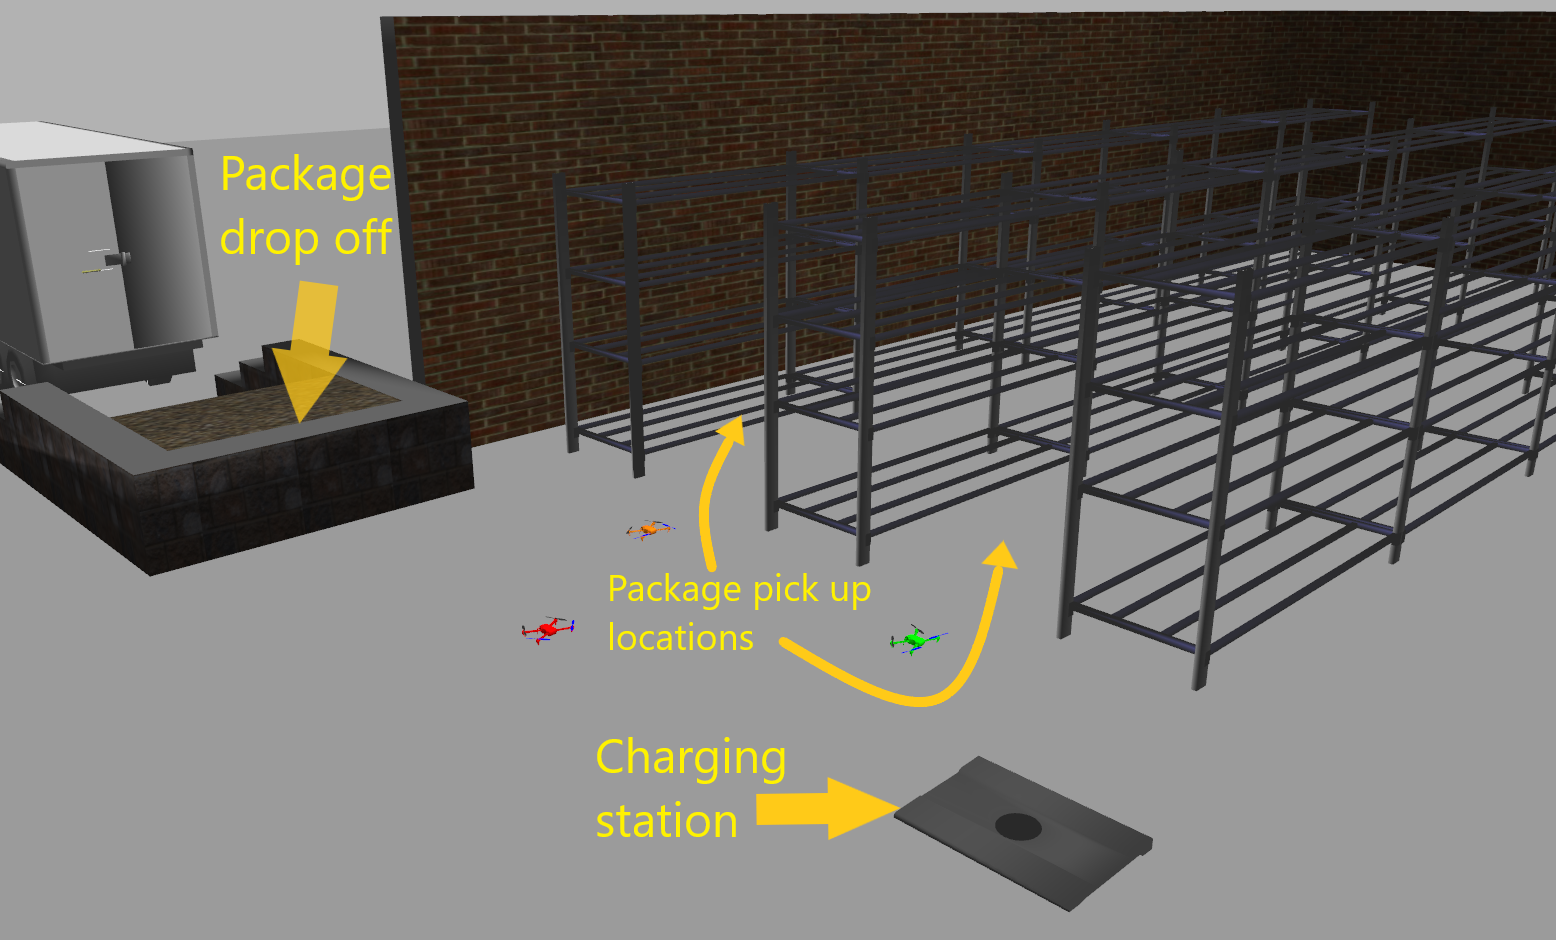
\includegraphics[width=0.95\textwidth]{MultiShield/figs/arenapicwithpad}
%\caption{Warehouse simulation environment in ROS.}
\label{fig:warehouse}
}
\hfill
\subfloat[Flowchart of the composed system.]{
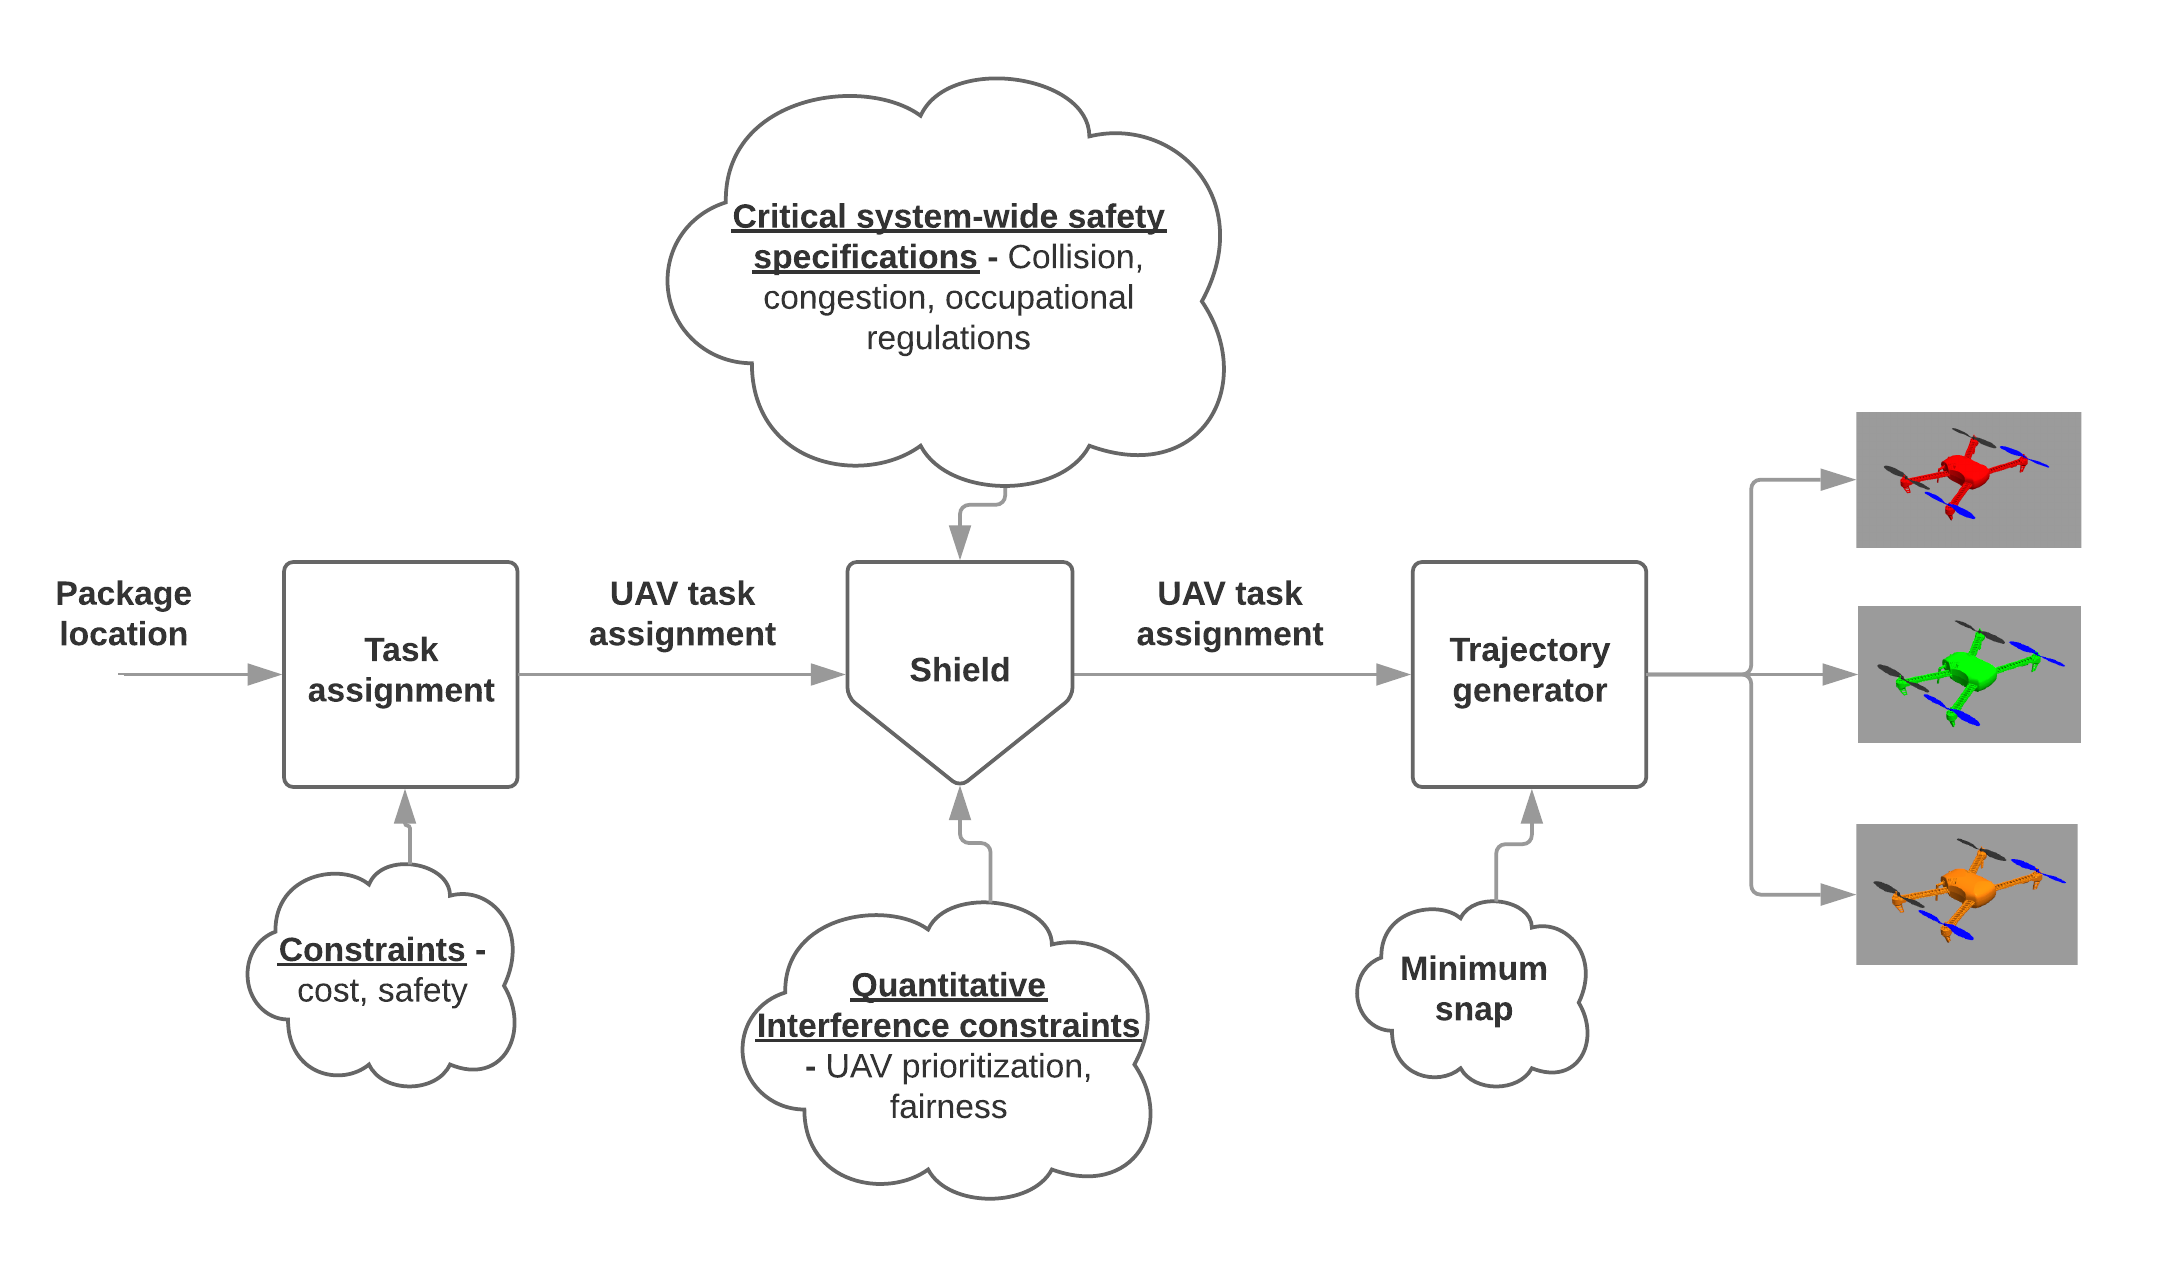
\includegraphics[width=0.995\textwidth]{MultiShield/figs/casestudy}
\label{fig:flowchart}}
\caption{Simulation environment and process workflow for three UAVs tasked with picking up packages off shelves and delivering them to the loading area.}
\label{fig:casestudy}
\end{figure}

The commands sent to move package(s) from the shelves to the loading dock are used to generate task assignments for the UAVs, and constitute the input to the system. The task assignment for the UAVs is sent either by a human operator who can command a particular UAV to perform a certain task, or by an automated system such as those in \cite{olivo2016method,kalyan2015automated}. To prevent congestion and collisions, global requirements for the multi-UAV system include not allowing more than one UAV in a given row at the same time, not allowing the UAVs to fly too close to each other, and not allowing UAVs to charge or drop of packages at the same time. 

The methods proposed in this paper can be used to synthesize a shield that enforces such  global safety properties and is agnostic to the nature of the system being protected. The shield takes the task assignment as an input and overwrites it with a new task assignment when necessary.  This is then sent to a trajectory generator which generates a minimum snap trajectory for each UAV to accomplish its task. In the following sections, we present the formalization of the multi-agent shielding problem, motivated in this example.
This process is summarized in Figure \ref{fig:flowchart}. 
 
 The safety specifications for this case study, and the results of the shield synthesis procedure are described and discussed in more detail in Section~\ref{sec:results_casestudy}.


%% \section{Shield formulation}
\subsection{Controller models}
\subsubsection*{Vertihub controller}We model the controller of each vertihub $V_i$ as a reactive system $\design_i = (\states_i,q_{0_i},\ialphabetx{i},\oalphabetx{i},\delta_{i},\lambda_{i})$ with input and output variables $I_i$ and $O_i$ respectively. The specific instantiation of such a controller is problem-specific, however, we present an illustrative example. 

% \begin{itemize}
%     \item $Q_i$ is a set of states,
%     \item the input alphabet $\ialphabetx{i}$ is the set of all possible environment inputs to the reactive controller,
%     \item the output alphabet $\oalphabetx{i}$ is the set of all possible control actions by the reactive controller,
%     \item the transition function $\delta_i$ maps the current state, environment input, controller output, to the next state,
%     \item the output function $\lambda_i$ maps the current state and environment input to a controller output.
% \end{itemize}
\begin{eg}
Consider the environment in Figure~\ref{fig:RegionsOutline} with vehicles moving between origin-destination vertiports. Each region $V_i$ is a vertihub with corresponding vertihub controller $\design_i$ where 
\begin{itemize}
    \item The state space $Q_i$ is the number of vehicles currently in the airspace of $V_i$, as well as the current delay time of any loitering vehicles in the airspace.
    \item $q_{0_i}$ is the starting airspace configuration of aircraft in $V_i$.
    \item The input alphabet is given by $\ialphabetx{i} = 2^{\inp_i}$. $\inp_i$ is the set of input variables and corresponds to \emph{requests} for the hub controller and the number of available landing slots in the region. We divide the requests into the following: landing, pass-through, take-off. 
    \item The output alphabet is given by $\oalphabetx{i} = 2^{\out_i}$. $\out_i$ is the set of output variables and corresponds to the following actions: allow vehicles to pass through, send vehicles to a vertiport in the region to land, or force vehicles to loiter until it is safe to allow them to enter. We note that the output can allow multiple requests to be granted simultaneously. 
    \item The transition function $\delta_i$ increments or decrements the number of vehicles and their corresponding delay times in the region based on the environment inputs and the resulting controller output. 
\end{itemize}
\end{eg}




Together, all $k$ vertihub controllers form a connected system which we define as set of reactive systems $\design = \{\design_1, \dots \design_k\}$ with a corresponding \emph{connectivity graph} $G_{\design}$.
We define a connectivity graph as a directed graph with each vertex corresponding to a reactive system.
We say two reactive systems are \emph{connected} if they share an edge in the graph. \textcolor{black}{ We define the set of reactive systems $\design_j \in \design$, $i \neq j$ that share an edge with $\design_i$ as $connect(\design_i)$.}
\begin{eg}
In Figure~\ref{fig:RegionsOutline}, overlapping operational regions share an edge in the corresponding directed graph in Figure~\ref{fig:Environment_directed} and therefore the corresponding reactive systems are connected. We say that $connect(\design_1) = \{\design_2,\design_3 \}$.
\end{eg}


Note that a hub controller forcing vehicles to loiter in the handoff region affects the connected hub controller.
For example, in Figure \ref{fig:RegionsOutline}, $\design_5$ forcing a vehicle loiter in $H_{56}$ affects the airspace of $\design_6$ and will as a result limit the number of vehicles that $\design_6$ can accept.
These handoffs necessitate the use of \emph{contracts} between hubs to guarantee the global system behaves as desired. 

\begin{figure}[h!]
	\centering
		\begin{tikzpicture}[auto,node distance=8mm,>=latex,font=\small]
        \tikzstyle{round} = [thick,draw=black,circle]
\tikzstyle{action} = [circle, draw, fill=black,inner sep=0pt, minimum size=4pt]
\node[round] (s1) {$\mathcal{T}_{1}$};
\node[round, right=15mm of s1] (s3){$\mathcal{T}_{3}$};
\node[round, below right=15mm and 5mm of s1] (s2){$\mathcal{T}_{2}$};
\node[round, right=15mm of s3] (s5){$\mathcal{T}_{5}$};
\node[round, right=10mm of s2] (s4){$\mathcal{T}_{4}$};
\node[round, right= 10mm of s5] (s6){$\mathcal{T}_{6}$};

\draw[<->] (s1) -- node[left]{$e_{12}$} (s2);
\path[<->,draw] (s1) -- node{$e_{13}$} (s3);
\path[<->,draw] (s2) -- node{$e_{23}$} (s3);
\path[<->,draw] (s2) -- node{$e_{24}$} (s4);
\path[<->,draw] (s3) -- node{$e_{34}$} (s4);
\path[<->,draw] (s3) -- node{$e_{35}$} (s5);
\path[<->,draw] (s4) -- node[right]{$e_{45}$} (s5);
\path[<->,draw] (s5) -- node[below]{$e_{56}$} (s6);

% \path[->,draw] (s1) edge[loop above] node {$e_{1}$} (s1);
% \path[->,draw] (s2) edge[loop below] node {$e_{2}$} (s2);
% \path[->,draw] (s3) edge[loop above] node {$e_{3}$} (s3);
% \path[->,draw] (s4) edge[loop below] node {$e_{4}$} (s4);
% \path[->,draw] (s5) edge[loop above] node {$e_{5}$} (s5);
% \path[->,draw] (s6) edge[loop above] node {$e_{6}$} (s6);

\end{tikzpicture}
\caption{The connectivity graph $G_\mathcal{T}$ of the UAM hub controllers $\mathcal{T}$ depicted in  Figure~\ref{fig:RegionsOutline}. 
Each edge $e_{ij}$ corresponds to $\mathcal{T}_i$ and  $\mathcal{T}_j$ being connected, i.e., the outputs of $\mathcal{T}_i$ are inputs to $\mathcal{T}_j$ and vice versa.}
\label{fig:Environment_directed}
\end{figure}


\subsubsection*{Vertiport controller} We assume without loss of generality that all regions $V_i$ contain $m$ vertiports. We model the \emph{vertiport controller} corresponding to region $V_i$ as a reactive system  $\shield_i^j = (\states^j_i,q^j_{0_i},\ialphabetx{i}^{j'},\oalphabetx{i}^j,\delta^j_i,\lambda^j_i)$ with $\states^j_i$ being the state space and $q^j_{0_i}$ being the initial state. The input alphabet $\ialphabetx{i}^{j'}$ is defined to be $\ialphabetx{i}^{j'} = \ialphabetx{j}^i\times \oalphabetx{i}$. This construction allows for the output of $\design_i$ to form part of the input for $\shield^i_j$ for $j = 1,\dots,m$. %Furthermore, the output of the vertiport controller feeds directly as input to the vertihub controller. Formally, $\out^j_i \subset \inp_i$. 

Figure \ref{fig:dist_shield} illustrates the relationship between hubs and vertiport controllers as well as the architecture of the composition. 


\begin{eg}
Continuing the running example based on Figure~\ref{fig:RegionsOutline}, each vertiport controller in the region $V_i$ has a corresponding set of input variables denoted $\inp_i^j$ and a resulting alphabet $\ialphabetx{i}^j$. This input corresponds to vehicles requesting to land that have been cleared by the corresponding vertihub controller  $\design_i$ and vehicles desiring to take off at one of its pads.
Hence, the output of $\design_i$ forms part of the input of $\shield^i_j$ for $j = 1,\dots,m$.
The output of the vertiport controller is the accepted or rejected take-off and landing requests as well as the number of remaining available landing pads which will then form part of the input to the hub controller. 
\end{eg}


%the outputs from the vertiport controllers feeding into the corresponding hub controllers. 

\begin{figure}[h!]
    % \hfill 
    \centering
		\newcommand{\OperatorSpaceT}[4]{
				%\draw[rounded corners = 15pt,dashed] (#1-#4,#2-#5) rectangle (#1+#4,#2+#5);
		\fill[fill=green,opacity=0.2] (#1,#2) circle (#3);
		\draw[draw = black,dashed](#1,#2) circle (#3);
		\node at (#1-#3-0.5,#2) {$\region_{#4}$};}
\newcommand{\Vertiports}[4]{
\fill[fill=black,opacity=1.0] (#1,#2) rectangle (#1+0.5,#2+0.5);
\node at (#1+1.0,#2) {$\shield^{#4}_{#3}$};
}

\newcommand{\LoopOver}[5]{
    \path[name intersections={of=#1 and #2}];
            \coordinate (S) at (intersection-1);
            \path[name path=circle] (S) circle(1.0mm);
            \path[name intersections={of = circle and #1}];
            \coordinate (I1) at (intersection-1);
            \coordinate (I2) at (intersection-2);
            \path[draw,very thick] (#3) -- (I1);
            \ifthenelse{#5=1}{\path[draw,very thick,->] (I2) -- (#4);}{\path[draw,very thick] (I2) -- (#4);}
            \tkzDrawArc[color=black,very thick](S,I2)(I1);
}


\definecolor{bodyyel}{HTML}{FFE58F}
\definecolor{bodybl}{HTML}{85A1DC}

    \subfloat[]{\scalebox{0.75}[0.65]{
    \begin{tikzpicture}[scale=0.55]
			\OperatorSpaceT{0}{0}{3}{2}
			\Vertiports{-1.5}{0.8}{1}{1}
			\Vertiports{0.6}{-1.2}{2}{1}
			\OperatorSpaceT{0}{-4.5}{3}{1}
			\Vertiports{0.25}{-6.2}{1}{2}
			
    \end{tikzpicture}
    }}
\quad
\subfloat[]{\scalebox{0.75}[0.65]{
    \begin{tikzpicture}
            \node[minimum width=1.5cm,rectangle,rounded corners,draw,minimum height=30mm,fill=yellow!20!white] (in) {$\ialphabetx{}$};
            
            
            \node[vert,right=10mm of in.60](vert1){$\shield^1_1$};
            \node[vert,right=10mm of in.40](vert2){$\shield^1_2$};
            \node[vert,right=10mm of in.315](vert3){$\shield^2_1$};
            \coordinate[left=10mm of vert1.205](in1);
            \coordinate[left=10mm of vert2.205](in2);
            \coordinate[left=10mm of vert3.145](in3);
            \coordinate[left=2mm of vert1](v1);
            \coordinate[left=2mm of vert3](v3);
            
            \node[vert,right=20mm of vert1,minimum height=10mm](S1){$S^1$};
            \node[vert,right=20mm of vert3,minimum height=10mm](S2){$S^2$};
            
            \node[hub,right=60mm of vert1] (hub1){$\design_1$};
            \node[hub,right=60mm of vert3] (hub2){$\design_2$};
            

            \path[name path=odest] (in1)--node[above] {} (vert1.205);
            
            \path[->,draw,very thick] (in2)--node[above] {} (vert2.205);
            \path[->,draw,very thick] (in3)--node[above] {} (vert3.145);
            
            \coordinate[right=20mm of vert1.30](c1);
            \coordinate[right=5mm of vert1.330](c2);
            
            % \path[draw,very thick] (vert1.30) |- (c1);
            \path[draw,very thick,->] (vert1.30) -- (c1);
            \path[name path=avail1] (vert1.330) |- (c2);
            % \path[name path=request2,very thick, draw] (vert2.30) -| (c1);
            \path[draw,very thick] (vert2.330) -| (c2);
            
            % \LoopOver{avail1}{request2}{vert1.330}{c2}{0};
            
            
            % \path[->,draw,very thick] (c1) -- node[above]{Ry} (S1.150);
            \path[->,draw,very thick] (c2) -- node[below]{} (S1.210);
            
            \coordinate[above right=10mm and 7.5mm of hub1](out1);
            \coordinate[below right=10mm and 5mm of hub2](out2);
            \path[draw,very thick] (hub1) -| (out1);
            \path[draw,very thick] (hub2) -| (out2);
            \path[->,draw,very thick] (vert3.east) -- (S2.west);
            % \path[->,draw,very thick] (vert3.30) -- node[above]{Rx} (S2.150);
            % \path[->,draw,very thick] (vert3.330) -- node[below]{Ax}  (S2.210);
            

            \coordinate[right=12.5mm of hub1.0] (loiter1);
            \coordinate[right=12.5mm of hub2.0] (loiter2);

            \coordinate[above left=10mm and 5mm of vert1.150] (X1);
            \coordinate[below left=10mm and 5mm of vert3.210] (X2);
            \coordinate[below right=5.5mm and 7.5mm of hub1](Y1);
            \coordinate[above right=6.5mm and 5.0mm of hub2 ](Y2);
            
            \path[->,draw, very thick] (hub1.0) --node[above right]{} (loiter1);
            \path[->,draw, very thick] (hub2.0) --node[above right]{} (loiter2);
            \path[draw, very thick] (out1) -- node[above,name=o1]{$\oalphabetx{1}$} (X1);
            \path[draw, very thick] (out2) -- node[below,name=o2]{$\oalphabetx{2}$} (X2);
            \path[->,draw,very thick](X1) |- (vert1.150);
            \path[->,draw,very thick,name path=land2](X1) |- (vert2.150);
            \path[->,draw,very thick](X2) |- (vert3.210);
            
            \path[draw,very thick] (hub1) -| node[below right] {} (Y1);
            \path[draw,very thick] (hub2) -| node[above right=5mm and 0mm] {} (Y2);
            \path[->,draw,very thick] (Y1) -| (hub2.120);
            \path[->,draw,very thick] (Y2) -| (hub1.280);
            
            \path[->,draw,very thick] (S1) -- node[above]{$\ialphabetx{1}$} (hub1);
            \path[->,draw,very thick] (S2) -- node[above]{$\ialphabetx{2}$} (hub2);
            
            
            \node[fit=(S1)(hub1)(vert1)(vert2)(v1),draw,dashed,minimum width=1.2cm,label={[above]$V^1$}]{};
            \node[fit=(S2)(hub2)(vert3)(v3),draw,dashed,minimum width=1.2cm,label={[below]$V^2$}]{};
            % \node[fit=(S2)(hub2)(vert3),draw,dashed,minimum width=1.2cm,label={[below]$V^2$}]{};
            \node [fit=(in)(o1)(loiter1)(o2),draw,dashed,label={[below right=5.5cm and 6cm of hub2]:{$V$}}] {};
            \LoopOver{odest}{land2}{in1}{vert1.205}{1};
            % \path[name intersections={of=odest and land2}];
            % \coordinate (S2) at (intersection-1);
            % \path[name path=circle2] (S2) circle(1.0mm);
            % \path[name intersections={of = circle2 and odest}];
            % \coordinate (I1) at (intersection-1);
            % \coordinate (I2) at (intersection-2);
            % \path[draw,very thick] (in.45) -- (I1);
            % \path[draw,very thick] (I2) -- (vert1.205);
            % \tkzDrawArc[color=black,very thick](S2,I1)(I2);
		\end{tikzpicture}
		}}

\caption{(a) Example region space with three vertiports and two operating regions with corresponding vertihubs and (b) Architecture of the composition of reactive systems. }
\label{fig:dist_shield}
\end{figure}
%As seen in Figure~\ref{fig:dist_shield}, the vertiport controller outputs the number of available landing slots to its corresponding hub controller.
In order for the reactive hub controller to be able to guarantee liveness properties, such as an upper bound on delay for all agents (a requirement), it needs to know the maximum time the vertiport controller will occupy a landing slot, i.e., it needs to know the worst case length of time a landing slot will be unavailable. 
Such an interaction between vertiport controller and hub controller is an example of a \emph{contract} and will be formally detailed in section~\ref{sec:distshield}.

\subsection{Controller composition}\label{sec:comp}
As mentioned previously, the inputs and outputs of the vertihub and vertiport controllers are linked. In this section, we formalize this notion by constructing the \emph{composition} of controllers.
We first define the composition of the $m$ vertiport controllers $\shield_i^j$ for all $j = 1,\dots,m$ corresponding to hub controller $\design_i$.
Formally, the vertiport controllers $\{\shield_i^1, \ldots,\shield_i^m\}$ in region $V_i$ can be composed as $\shield_i = \shield_i^1 \comp \ldots \comp \shield_i^m$. %\textcolor{magenta}{Is it intentional that you define the compsition as $S_i$, but the reactive system as $S^i$ in the next sentence?}
The resulting composition is also a reactive system
$\shield^i=(\overline{\states}_i, \overline{q}_{0_i},\overline{\Sigma}_{\inp_i}, \overline{\Sigma}_{\out_i}, \overline{\delta}_i, \overline{\lambda}_i)$ defined as follows:
\begin{itemize}
    \item the set $\overline{\states}_i = \bigotimes_j \states_i^j$ of states is formed by the product of the states of all vertiports $\shield^i_j \in \shield^i$.
    \item The initial state $\overline{q}_{0}$ is formed by the initial states $q_{0_i}^j$ of all $\shield_i^j \in \shield^i$.
    \item The input alphabet $\overline{\Sigma}_{\inp_i}$ is given by $\overline{\Sigma}_{\inp_i}  = \bigotimes_{j=1}^m \ialphabetx{i}^{j'}$.
    \item The output alphabet $\overline{\Sigma}_{\out_i},$ of the joint system  $\shield^i$ is given by $\overline{\Sigma}_{\out_i} = \bigotimes_{j=1}^m \oalphabetx{i}^j$.
    \item The transition function $\overline{\delta}_i$ updates, for each vertiport controller $\shield_i^j \in \shield_i$, the $\states^j_i$ part of the state 
    in accordance with the transition function $\delta^j_i$.
%the projection $\symb(I_j)$ as input.
\item The output function $\overline{\lambda}_i$ labels each state with the union of the outputs of all $\shield^i_j \in \shield^i$ according to $\lambda^j_i$.
\end{itemize}

%
% While multiple vertiports may be able to read the same input variables to indicate
% broadcast from the vertihub controller, the sets of outputs are pairwise disjoint. %: for $k \neq j$, we have $\out_k \cap \out_j = \emptyset$.
% %Furthermore, vertiports cannot directly read each others outputs, that is, for all $k$ and $j$, we have $\out_k \cap \out_j = \emptyset$.
% The output alphabet of the joint system  $\shield^i$ is given by $\oalphabetx{i}' = \bigotimes_{j=1}^m \oalphabetx{i}^j$, and the input alphabet is given by $\ialphabetx{i}'  = \bigotimes_{j=1}^m \ialphabetx{i}^{j'}$.
% %
% The joint behaviour of the composed vertiport system is a reactive system 
% $\shield^i=(\states, q_{0}, \ialphabet,\oalphabet, \delta,\lambda)$ defined as follows: 






Next, we define the composition of the joint vertiport controllers $\shield^i$ %\textcolor{magenta}{[note that in the composition definition below you use $S_i$ to denote the vertiport controller composition]} and the corresponding hub controller $\design_i$. 
Formally, we compose the two systems in serial fashion in the following way: $\design_i \comp \shield_i := \mathcal V_i =
(\hat{\states}_i, \hat{q}_{0_i}, \hat{\Sigma}_{\inp},\oalphabetx{i}, \hat{\delta}_i,
\hat{\lambda}_i)$, with 
\begin{itemize}
    \item states $\hat{\states}_i = \states_i \times \overline{\states}_i$,
    $\hat{q_{0}}_i = (q_{0_i},\overline{q}_{0_i})$,
    \item input alphabet $\hat{\Sigma}_{\inp} = \ialphabetx{i} \times \overline{\Sigma}_{\out_i}$,
    \item transition function $$\hat{\delta_i}((q_i,\overline{q}_i),\hat{\sigma}_\inp) = (\delta_i(q_i,\isymbx{i}),\overline{\delta}_i(\overline{q}_i,(\overline{\sigma}_{\out_i},\isymbx{i}))),$$
    \item and output function $$\hat{\lambda}_i((q_i,\overline{q}_i),\hat{\sigma}_\inp) = \lambda_i(q_i,(\isymbx{i},\overline{\lambda}_{i}(\overline{q}_i,\overline{\sigma}_{i}))).$$ 
\end{itemize}
   
    
    
   Note that, by construction, the output alphabet of the composition $\oalphabetx{i}$ is the same as that of the hub controller.
   

Finally, the \emph{global system} $ \mathcal V = \{ \mathcal V_1 \dots \mathcal V_k \}$ is the composition of all $V_i$ and the definition proceeds analogously to the composition of the vertiports. The architecture of the defined composition in an example environment with two hub controllers is illustrated in Figure \ref{fig:dist_shield}. We remark that the \emph{global composition} is of the form of a multi-agent reactive system as studied in \cite{multiagentshield}.

In the next 2 subsections, we define the properties that we want the global system to satisfy and formally define the synthesis problem.
In Section \ref{sec:distshield}, we present our synthesis procedure for the vertiport and hub controllers and prove the global system stemming from their composition will satisfy all required properties. 



\subsection{Specifications}\label{sec:specs}
Recall that each hub controller is required to satisfy a user provided specification. Formally, the specification for hub controller $\design_i$ must be of the form 

\begin{equation}\label{eq:formalspechub}
    \varphi_{\design_i} = \LTLglobally S_i \wedge \LTLglobally \LTLfinally P_i
\end{equation}

\noindent where $S_i, P_i \subseteq Q_i$. 

Similarly, each vertiport controller must also satisfy its own user-provided specification, and is defined the same way. For vertiport controller $\shield^j_i$ we have $\varphi_{\shield^{j}_i} = \LTLglobally S_{i}^j \wedge \LTLglobally \LTLfinally P_{i}^j$ where $S_{i}^j, P_{i}^j \subseteq Q_i^j$. 

For each region $V_i$, we denote the conjunction of all the vertiport specifications $\varphi_{\shield^{j}_i}$ for $j=1,\ldots,m$ with the corresponding vertihub specification $\varphi_{\design_i}$ as $\varphi_i := \varphi_{\design_i} \bigwedge \left( \varphi_{\shield^{1}_i} \wedge \ldots \wedge 
\varphi_{\shield^{m}_i}\right)$. 

\begin{eg}
A simple example of a specification in the form of~\eqref{eq:formalspechub} can be $\LTLglobally \left(\text{fewer than N vehicles in region} \right) \wedge \LTLglobally\LTLfinally (\text{vehicle request is granted})$. Informally, such a specification requires that no more than $N$ vehicles be in the region at any given time and that always eventually any vehicle is allowed to pass-through or land in the region if they request it, i.e., they cannot be made to wait forever. 
\end{eg}


\subsection{Synthesis problem}\label{sec_correctness}

Now we define the basic  requirements that the overall composed system must satisfy: namely it should enforce correctness with respect to a given user specification.
Informally, this translates to enforcing safety while guaranteeing progress. 

% \paragraph{\textbf{No unnecessary interference}}
% A shield is only allowed to interfere when the output of the reactive system  is not \emph{correct}.
% %
% Formally, given a safety specification $\spec$, a reactive system $\shield = (\states',q_{0}',\ialphabet'\times\oalphabet',\oalphabet,\delta',\lambda'$ \emph{does not interfere unnecessarily} if for any reactive system
% $\design = (\states,q_{0},\ialphabet,\oalphabet,\delta,\lambda)$ and any trace
% $(\itrace\parallel\otrace)\in (\ialphabet \times \oalphabet)^\infty$
% of $\design$ that is not wrong, we have that $\shield(\itrace \parallel  \otrace) = \otrace$.

% \begin{definition}
% A \emph{shield} for a given safety specification $\spec$ is a reactive system $\shield = (\states,q_{0},\ialphabet\times\oalphabet,\oalphabet,\delta,\lambda)$
% such that for any reactive system $\design = (\states,q_{0},\ialphabet,\oalphabet,\delta,\lambda)$ it holds that $(\design \comp \shield) \models \spec$ and $\shield$  does not deviate from $\design$ unnecessarily.
% \end{definition}

% \begin{definition}
% A set of localized \emph{shields} $\shield = [\shield_1 \cdots \shield_n]$ for a conjunction of specifications $\spec = \bigwedge_i^n \spec $ is a set of reactive systems such that for $\shield_i \in \shield$, where $\shield_i = (\states',q_{0}',\overline{\ialphabet}_i\times\oalphabetx{i},\oalphabetx{i},\delta',\lambda')$,
% for any set of connected reactive systems $\design = [\design_1 \cdots \design_n]$ where $\design_i = (\states_i,q_{0_i},\ialphabetx{i},\oalphabetx{i},\delta_i,\lambda_i)$ with connectivity graph $G_{\design}$, it holds that $\design_i \comp \shield_i \models \spec_i$ with no unnecessary deviation. Additionally, it must hold that the global composition is correct with respect to the conjunction of specifications. Formally, $(\design_1\comp \shield_1) \comp \cdots \comp (\design_n\comp \shield_n) \models \varphi_1 \wedge \cdots \wedge \varphi_n$.
% \end{definition}

% \subsection{Safety shield formulation}\label{sec:caseshield}

% The goal is to ensure the successful transition of each UAV to its corresponding goal location or without the violation of any safety requirements. If a UAV needs to pass through an operator's region, the shield needs to assess if this is allowed and act accordingly. We require that shield not allow violation of safety specifications as well as guaranteeing that every UAV that wants to pass through its region is eventually allowed to do so. We give the shield the power to do the following:
% \begin{itemize}
%     \item Make UAVs wait/loiter before entering its region (for a prescribed maximum amount of time).
%     \item Force UAVs to leave the region, but without causing the disruption of currently executing tasks. 
% \end{itemize}
% In order to give the required guarantees we will need to make assumptions on the behaviour of the shields of neighbouring regions. We cover this in more detail in Section \ref{sec:distshield}. 

% \subsection{Safety specifications}
% This overall system must abide by a set of \emph{global} safety specifications given in LTL by $\varphi_g$. We are interested in employing a \emph{separation of concerns} approach between the MDP and the shields. Hence, we assume that $\varphi_g$ can be divided into into a conjunction of two classes of specifications $\varphi_g = \varphi_r \wedge \varphi_f$. 

% The shields handle \emph{region-specific} requirements $\varphi_r$. An example of such a specification can include not allowing more than a certain number of UAVs to operate within their region at any given time. This can vary from region to region and is thus under purview of the respective shield. Given $n$ regions (in Figure~\ref{fig:RegionsOutline} $n=6$), we represent $\varphi_r$ as a conjunction of region-specific specifications, i.e.  $\varphi_r = \bigwedge_{i=1}^n\varphi_i$. 

% The second class of requirements, which we denote as $\varphi_f$ are \emph{route-based} requirements. An example of such a requirement may be not allowing too many UAVs to pass through the same region at the same time on their route.  Since these involve UAVs coordinating across multiple regions, the shield of each region cannot be responsible for the satisfaction of such specifications as each shield can only observe UAVs within its region. We will require the UAV routes be computed in a decentralized manner, and thus they will need to dynamically coordinate at run-time to avoid the violation of such specifications. 

Given (1) environment structure with $k$ vertihubs, (2) $m$ corresponding vertiports for each hub, (3) hub connectivity graph $G_D$, and (4) GR(1) specifications $\varphi_{\design_1},\dots, \varphi_{\design_k}$ for each vertihub and vertiport specifications $\varphi_{\shield_i^j}$ for all $i = 1,\ldots,k$ and $j=1,\ldots,m$ synthesize a set of hub controllers $\design = [\design_1, \ldots, \design_k]$ and their corresponding vertiport controllers $\shield^i_j$ for all $i = 1,\dots, k$ and $j = 1,\dots, m$ such that the global composition of all controllers is \emph{winning} with respect to $\bigwedge_{i=1\dots k}\varphi_i$.
Formally, synthesize hub and vertiport controllers such that:
\begin{equation}\label{eq:problem}
\left( \design_1 \comp \left( S_1^1 \comp \dots S_1^m \right) \right) \comp \dots \left( \design_k \comp \left( S_k^1 \comp \dots S_k^m \right) \right) \models \bigwedge_{i=1\dots k}\varphi_i
\end{equation}





% synthesize a set of localized shields $\shield = [\shield_1 \cdots \shield_n]$ for any set of reactive systems $\design = [\design_1 \cdots \design_n]$ with connectivity graph $G_{\design}$, such that each $\shield_i$ is (1) correct with respect to $\spec_i$, (2) can only correct the outputs of $\design_i$, (3) can only observe the outputs of sectors in $connect(\design_i)$, and (4) global composition of the shields and design is correct with respect to the conjunction of safety specifications. Informally (4) states that $\shield_i$ must not only be correct with respect to $\spec_i$, but also must not prevent all connected shields from satisfying their safety specifications.

%\hasan{The problem statement hides the complex situation where $\spec_i$ depends on states/propositions from all regions, yet the shield can only limit actions from one region. Maybe add a remark here? NATASHA ADDS:  excellent point, as safety is an emergent system property, and thus depends on the total state.}

In the next section, we present the decentralized contract-based synthesis framework to generate the controllers. 




\section{Decentralized controller synthesis framework}\label{sec:distshield}
%In this section, we present a correct-by-design approach to decentralized controller synthesis with assume-guarantee contracts.
We first formalize the notion of assume-guarantee contracts, then we demonstrate the incorporation of these contracts as a GR(1) winning condition to a two-player game, which we solve using reactive synthesis~\cite{Piterman06,bloem2012}. 

\subsection{Assume-guarantee contracts}

We employ a decentralized synthesis process. Each controller is synthesized without an awareness of the specification and implementation details of both the vehicles in the fleet as well as the controllers in connected vertihubs.
However, a vertihub controller's outputs impact the controllers of its neighboring vertihubs. 
In order to ensure that controllers don't hinder each others' abilities to satisfy their local specifications, every controller must additionally satisfy \emph{contract specifications} for each neighboring vertihub.
Similarly, all vertiport controllers impact the implementation of their corresponding vertihub controllers. Therefore, the vertiport controllers must also satisfy contract specifications with their hub controller and vice versa. 

 These contract specifications take the form of \emph{assume-guarantee} contracts. 
 Informally, a vertihub controller gives a \emph{guarantee} of satisfying a contract specification with a neighboring vertihub controller.
 This guarantee is used as an assumption for the synthesis of the neighboring controller and vice-versa.
 These contract specifications are taken into account in the synthesis process for all controllers. 
% An assume-guarantee contract for a controller expresses the assumptions on the connected controllers' outputs and the guarantees on the corresponding controller's outputs. 


 
 In this setting, we introduce two classes of contracts: contracts between connected vertihub controllers and contracts between a vertihub and its corresponding vertiport controllers. 
 
 \subsubsection{Vertihub controller contracts}
% For ease of notation, the following definitions are with respect to the assumptions and guarantees of the $i^{th}$ hub controller. 
 An \emph{assume-guarantee contract} for a vertihub controller $\design_i$ with connected hub controller $\design_j$ is a tuple $\mathcal \phi_{\design_i}^{\design_j} = (A_{\design_i}^{\design_j},B_{\design_i}^{\design_j})$ where:
\begin{itemize}
\item $A_{\design_i}^{\design_j}$ is an assumption on the outputs of $\design_j$ as it pertains to ${\design_i}$ expressed as a specification in the form shown in Equation ~\eqref{eq:formalspechub}. 
\item $B_{\design_i}^{\design_j}$ is a specification also in the form shown in Equation ~\eqref{eq:formalspechub}  which $\design_i$ must guarantee on the outputs pertaining to $\design_j$.
\end{itemize}
Similarly, the contract for $\design_j$ with $\design_i$ is denoted $\mathcal \phi_{\design_j}^{\design_i} = (A_{\design_j}^{\design_i},B_{\design_j}^{\design_i})$.


\begin{eg}
Consider Figure~\ref{fig:dist_shield}. An example of a contract that $\design_1$ will make with $\design_2$ is an upper bound on the length of time $\design_1$ can refuse to accept vehicles from $\design_2$ when requested. Such a contract is expressed as $\phi_{\design_2}^{\design_1}= (A_{\design_2}^{\design_1},B_{\design_2}^{\design_1})$ where $A_{\design_2}^{\design_1} = B_{\design_2}^{\design_1} = \LTLglobally \left(\text{delay } \leq \text{ T}\right)$ for some integer value $T$. Hence, the controller $\design_1$, in addition to satisfying its local specifications, must also guarantee $B_{\design_2}^{\design_1}$, i.e., it does not keep an aircraft from $\design_2$ waiting for more than $T$ timesteps. In order to help satisfy the additional specification, $\design_1$ makes the assumption $A_{\design_2}^{\design_1}$ that $\design_2$ will satisfy $B_{\design_1}^{\design_2}$. Recall that the user given specification for $\design_1$ is denoted $\varphi_{\design_1}$. Under this contract, the augmented requirement $\varphi_{\design_1}'$ for $\design_1$ is
$$ \varphi_{\design_1}' := A_{\design_2}^{\design_1} \implies \varphi_{\design_1} \wedge B_{\design_2}^{\design_1} $$
Simply, if the assumption on $\design_2$ holds, then the original specification must be satisfied in addition to contract specification $B_{\design_2}^{\design_1}$. The same procedure follows for $\design_2$. \end{eg}


\subsubsection{Vertiport controller contracts}
Each vertihub controller must also make contracts with the vertiport controllers in its region. The procedure follows analogously as in the previous section, as it is assumed that all outputs from the individual controllers are \emph{pairwise disjoint}. Hence, we form separate contracts with each vertiport controller. Formally, we define a contract between a vertihub controller $\design_i$ and one of its vertiport controllers $\shield_i^j$ as $ \phi_{\shield^j_i}^{\design_i} = (A_{\shield_i^j}^{\design_i},B_{\shield_i^j}^{\design_i})$ where $(A_{\shield_i^j}^{\design_i},B_{\shield_i^j}^{\design_i})$ are, analogous to the hub contracts, the respective assumptions and guarantees on the vertiport controller, expressed as temporal logic specifications of the form in~\eqref{eq:formalspechub}. 

\subsubsection{Symmetric contracts}
We say contracts between two reactive systems $\design_i$ and $\design_j$ denoted by $\phi_{\design_i}^{\design_j}  $ and $\phi_{\design_j}^{\design_i}$ are \emph{symmetric} if $A_{\design_i}^{\design_j} = B_{\design_j}^{\design_i}$ and $A_{\design_j}^{\design_i} = B_{\design_i}^{\design_j}$. 

Informally, this means that the assumptions $\design_i$ makes on the outputs of $\design_j$ corresponds to the \emph{guarantees} $\design_j$ gives on its own outputs. All the contracts we will use in the synthesis procedure will be symmetric, as this will guarantee that the assumptions each reactive system makes on the outputs of other systems will actually hold. 

\subsubsection{Joint winning condition}
The addition of the contract specifications to the original user-provided specifications modifies the winning condition presented in~\eqref{eq:problem}. The following lemma presents the modified winning condition for hub controller $\design_i$ when contracts are incorporated. 
\begin{lemma}
For a set of vertihub controllers $\design$, hub connectivity graph $G_\design$, the winning condition for controller $\design_i \in \design$ with the set of vertiport controllers $\shield_i^j$ for $j = 1,\ldots,m$ is given by
\begin{equation}\label{eq:contractproblem}
     \varphi_{i}' := \left( \bigwedge_{j=1}^{m} A_{\shield_i^j}^{\design_i} \bigwedge_{\design_j\in J} A_{\design_j}^{\design_i} \implies \varphi_{\design_i} \wedge B_{\shield^i}^{\design_i} \bigwedge_{\design_j\in J} B_{\design_j}^{\design_i} \right)
\end{equation}
where $J = connect(\design_i)$.
\end{lemma}
% \begin{proof}
% Follows from the construction of $\varphi_{\design_i}$.
% \end{proof}
\textcolor{black}{Note that~\eqref{eq:contractproblem} is in the same form as the specifications in~\eqref{eq:formalspechub} which allows us to use efficient GR(1) synthesis techniques~\cite{bloem2012}.} We state this formally in the following lemma. 
\begin{lemma}\label{lemma:gr1}
The winning condition in \eqref{eq:contractproblem} is GR(1).
\end{lemma}


\paragraph*{\textbf{Remark}} We note that the values in the assume-guarantee contracts are heavily dependent on the topology of the environment and the connections. For example, a hub with many connecting hubs may not be able to guarantee quick transit of vehicles through its regions. Generating these contracts automatically based on the given graph $G_{\design}$ is a subject of future work. In this dissertation, the contract values are chosen manually. 


\subsection{Controller synthesis}
We first present an overview of the synthesis procedure. Informally, we avoid the centralized synthesis problem by creating a series of smaller synthesis problems that are connected through the architecture and contract specifications introduced earlier.
The synthesis procedure for a vertihub controller $\design_i$ consists of the following steps:
\begin{itemize}
 \item[1)] First, we synthesize all the vertiport controllers $\shield_i^j$ for $j=1,\ldots,m$ operating under $\design_i$. For each controller $\shield_i^j$ we construct a game $\game_{i}^j$ with the acceptance condition given by the user-provided specification $\varphi_{\shield_i^j}$. We then augment the acceptance condition to include the contract specification $\phi_{\shield_i^j}^{\design_i}$. 
  \item[2)] As shown in Lemma~\ref{lemma:gr1}, the winning condition stemming from augmenting $\varphi_i$ with the contract specifications is a GR(1) condition. We solve each game $\game_{i}^j$ using GR(1) reactive synthesis~\cite{bloem2012}. 
  \item[3)] We compose the joint vertiport controllers to form $\shield_i$. We construct a game $\game_{i}$ from the given specification $\varphi_{\design_i}$ for the vertihub controller $\design_i$, again augmenting the acceptance condition with the vertiport contract specifications $\phi^{\shield_i^1}_{\design_i} \wedge \ldots \wedge \phi^{\shield_i^m}_{\design_i}$. We now additionally augment the acceptance condition with contract specifications $\phi_{\design_i}^{\design_j}$ from all connected vertihub controllers $\design_j \in connect(\design_i)$. Similar to before, this results in another GR(1) acceptance condition and we can compute a winning strategy. 
\item[4)] The process is repeated for each hub controller.
\end{itemize}

%In the following subsections we present the synthesis of the shield $\shield_i$. For notational clarity we omit the subscript $i$ in the following description. 


\subsubsection{Game construction}
Recall that computing the output function $\lambda_i$ corresponding to the reactive system $\design_i$ is framed as finding the winning strategy obtained from solving a game. The game construction is identical for the vertiport and vertihub controllers, just with different specifications and contracts. For brevity, we present the game construction for the synthesis for vertihub controller $\design_i$.

Let $\varphi_{\design_i} = \LTLglobally S_i \wedge \LTLglobally \LTLfinally P_i$ with $P_i,S_i \in Q_i$ be the user-provided specification for reactive system $\design_i = (Q_i,q_{0_i},\ialphabetx{i},\oalphabetx{i},\delta_i,\lambda_i)$. The corresponding game $\game$ is constructed as follows: $\game = \left(Q,q_0, \alphabet, \delta,\Acc \right)$
where $Q = Q_i$, $q_{0} = q_{0_i}$, $\alphabet = (\ialphabetx{i} \times \oalphabetx{i})$, $\delta = \delta_i$, and $\Acc$ is the winning condition presented in Equation~\eqref{eq:contractproblem}. 
The task is to synthesize a strategy $\rho$ that maps the current state $q_i$ and environment input $\sigma_i$ to an action $\sigma_0$ such that for all possible input sequences $\sigma_i \in \ialphabetx{i}^*$ we will have $\Acc(\pi) = \top$.
From Lemma~\ref{lemma:gr1}, we know that $\Acc$ is a GR(1) winning condition. Hence, we are able to use the techniques in~\cite{bloem2012} in order to efficiently synthesize a strategy $\rho: Q\times\ialphabetx{i} \rightarrow \oalphabetx{i}$. Setting the output function $\lambda_i$ corresponding to hub controller $\design_i$ to be the winning strategy $\rho$ for game $\game$ as defined above  leads to the following lemma. 
\begin{lemma}
$\design_i \models \varphi_i$ if $\rho \models \varphi_i'$ and $ \left(\bigwedge_{j=1}^m A_{\shield_i^j}^{\design_i} \bigwedge_{\design_j\in J} A_{\design_j}^{\design_i} \right)$ holds. 
\end{lemma}
\paragraph{Proof sketch}:
The proof relies on the game construction having an identical state space as the reactive system and the definition of $\varphi_i'$ being \emph{both} the original user-provided specification $\varphi_i$ as well as the contract specification. Since the game strategy satisfies $\varphi_i'$, then the same strategy must also satisfy $\varphi$ iff the assumptions made on neighboring vertihubs and interior vertiports are satisfied.
\textcolor{black}{Informally, the lemma states that the hub controller $\design_i$ satisfies its given specification $\varphi_i$ if the synthesized strategy $\rho$ from the game $\game$ is winning with respect to the contract augmented specification $\varphi_i'$ and the contract assumptions hold.}
\paragraph*{\textbf{Remark}} The above lemma is only a statement of \emph{sufficiency}. This is because the contract specifications that form $\varphi_i'$ are not unique. If $\rho \nvDash \varphi_i'$, for a particular set of contracts, this does not mean there does not exist a $\lambda_i$ such that $\design_i \models \varphi$.




%  For each $\shield_i$, we construct a game $\mathcal G^{\shield_i}$ such that its most permissive strategy subsumes all possible shields that are correct w.r.t.\ $\varphi_i$ and the contract safety guarantees, given that the contract safety assumptions hold.
% %
% Let $J$ be the set of indices of sectors connected to $\shield_i$.
% We first define two boolean variables $t_j$ and $u_j$  for all $j \in J$:
% \begin{itemize}
%     \item $t_j$ is true when a vehicle attempts to move from the sector shielded by $\shield_j$ to the sector of $\shield_i$, and $\shield_i$ does not allow it to enter. 
%     \item $u_j$ is true when $\shield_i$ attempts to move a vehicle to a sector shielded by $\shield_j$ and $\shield_j$ does not allow it to enter. 
% \end{itemize}
% %\rayna{Who controls the variables $t_j$ and $u_j$? It appears that they encode both the desire of a UV/shield to move the UV, and the decision of the other shield to disallow this.}\suda{$t_j$ is a system variable and $u_j$ is an environment variable. The assumption is then encoded in slugs as a safety property in $u_j$}
%  Given the contracts $C^{\shield_i}_{\shield_j}$, the shield must additionally satisfy contract-induced safety guarantees $B^{\shield_i}_{\shield_j}$ given assumptions $A_{\shield_i}^{\shield_j}$. To encode these contracts, the state space $G^{\shield_i}$ of $\mathcal G^{\shield_i}$ is constructed by augmenting the states $Q$ of $\varphi$ with two tuples of integer variables: $(v_j)$ and $(w_j)$  for all $j \in J$, as is explained below.
 
% %  \hasan{$B^{\shield_i}_{\shield_j}$ is not a true safety specification, but one we make up to enable distribution of shielding. Is that correct?}\suda{It is one we make up in order to guarantee the synthesis problem is realizable. It is still a 'true' safety spec though. But not 'true' in the sense that the problem statement demands it. Perhaps artificial safety spec is the right word to use.} \hasan{How about induced, contract-induced, \textbf{contractual}, or conditional safety specifications?} 

% We construct a game $\mathcal G^{\shield_i} = (G^{\shield_i}, g_0^{\shield_i}, \ialphabet,\oalphabet,\delta^{\shield_i}, \Acc^{\shield_i})$ such that 
% $G^{\shield_i} = \{(g\bigotimes_j (v_j,w_j) \mid g \in Q, j\in J\}$ is the state space,
% % $G^s = \{(g,(v_j),(w_j)) \mid g \in Q, j\in J\}$ is the state space,
% $g_0^s = (g_0,(0,0),\ldots,(0,0))$ is the initial state %\natasha{hmmm...I don't know if there is any better way to indicate that there are as many (0,0) tuples as their are neigboring sectors.  Maybe it is obvious.},
% $\delta^s$ is the next-state function, such that
% $\delta^s((g,(v_j,w_j)),( \isymb,\osymb),\osymb')=(\delta(g, \isymb,\osymb'),(v_j',w_j'))$ 
% %\natasha{Have we explained the difference between $\osymb'$ and $\osymb$?  Or do we not need to?}\suda{Former is the output of the sector controller and the latter is the shield output. This should be explained in section 3}
% with
% \begin{itemize}
% \item if $v_j \leq b^{\shield_i}_{\shield_j}$, $t_j'=\top$, then $v_j' = v_j+1$,
% \item if $v_j \leq b^{\shield_i}_{\shield_j}$, and $t_j'=\bot$, then $v_j'= 0$,
% \item if $v_j = b^{\shield_i}_{\shield_j} +1$, then $v_j' =b^{\shield_i}_{\shield_j}+1$
% \item if $w_j \leq a^{\shield_i}_{\shield_j}$, and $u_j'=\top$, then $w_j' = w_j+1$,
% \item if $w_j \leq a^{\shield_i}_{\shield_j}$and $t_j'=\bot$, then $w_j' = 0$
% \item if $w_j = a^{\shield_i}_{\shield_j} +1$, then $w_j' =a^{\shield_i}_{\shield_j}+1$; 
% \end{itemize}
% for all $j \in J$,
% % and $F^s=\{(g,(v_j,w_j))\in G^s \mid (g\in W) \bigwedge_j \left((v_j\leq  B^{\shield_i}_{\shield_j})\vee (w_j >   A^{\shield_i}_{\shield_j})\right),  j \in J \}$.
% and $\Acc^{\shield_i}$ is such that  $\Acc^{\shield_i}(\overline{\pi})=\top$ iff\looseness=-1
% \begin{itemize}
% \item $\exists t \geq 0 \scope g_t^{\shield_i}= (g_t,(v_{j_t},w_{j_t}))$ with $w_{j_t} > a^{\shield_i}_{\shield_j}$, or

% \item there are inf. many $g_t^{\shield_i}= (g_t,(v_{j_t},w_{j_t}))$ with $ \bigwedge_j v_{j_t} \leq b^{\shield_i}_{\shield_j}$ for all $j\in J$.
% \end{itemize} 

% Intuitively, the counter $w_j$ tracks the number of consecutive times $\shield_j$ refuses to accept a vehicle, and is reset to $0$ when the vehicle is accepted. If $w_j$ exceeds the bound $ A^{\shield_i}_{\shield_j}+1$, it remains $ A^{\shield_i}_{\shield_j}+1$ forever.
% Using this counter $w_j$, we encode the assumption $\shield_i$ makes on the behaviour of $\shield_j$. 
% Similarly, the counter $v_j$ tracks the number of consecutive times $\shield_i$ refuses to accept a vehicle from $\shield_j$ and is reset to $0$ when a vehicle is accepted. We use $v_j$ to encode the guarantee $\shield_i$ must give to $\shield_j$. We note that encoding the integers in this manner means $\Acc^{\shield_i}$ is a safety acceptance condition and $\mathcal{G}^{\shield_i}$ is a safety game.

% %We note that we have implicitly assumed without loss of generality only one vehicle from each sector can transit to a neighbouring sector at a time 


% % \begin{itemize}
% % \item if $v_j \leq k_{\shield_j}$, $w_j \leq f_{\shield_j}$ and $t_j'=\top$, then $v_j' = v_j+1$, $w_j' = 0$,
% % \item if $v_j \leq k_{\shield_j}$, $w_j \leq f_{\shield_j}$ and $t_j'=\bot$, then $v_j'= 0$, and $w_j' = w_j+1$ \natasha{are we using the bottom symbol to signify false?}
% % \item if $v_j = k_{\shield_j} +1$, then $v_j' =k_{\shield_j}+1$
% % \item if $w_j = f_{\shield_j}+1$ and $t_j'=\bot$, then $w_j' = f_{\shield_j}$; 
% % \end{itemize}
% % \natasha{Have we made some kind of implicit assumption in the persistence of the request?  That is, once a shield requests transit, it continues to request transit until the UVs have fully transited?  Or presumably there is some form of controller in the sector that makes sure that UVs don't get shuttled from border to border, requesting access into differing neighboring sectors in a periodic fashion, thereby trapping them in the sector indefinitely?}\suda{There is an implicit assumption that the the controller does not shuttle the UVs from border to border. Implicitly, when a UV requests to leave a region, the shield of the region it wants to enter assumes 'control'. The shield only has the power to force loiter of entering UVs, so UVs will not be shipped from border to border. The region the UV is currently in does not care what happens to the UV as it leaving the region on its own accord is the best case scenario for the shield. }
% We use standard algorithms for safety games (e.g.~\cite{Mazala01})
% to compute the winning region $W^s$ and the most permissive winning strategy $\rho^s: G \times \ialphabet \rightarrow 2^{\oalphabet}$ of $\mathcal G^s$. 


\subsection{Correctness}
In this section we present the correctness result that states that if there exists a set of controllers  synthesized using the construction detailed earlier, they must be winning with respect to the conjunction of all user provided specifications.  
\begin{thm}
If there exists a set of controllers $\design = [ \design_1,  \dots, \design_k ]$ with corresponding vertiport controllers $\shield^j_i$ for $j=1,\dots,m$ and $i=1,\dots,k$ such that $\design_i \models \varphi_i'$  where $\varphi_i'$ is given in Equation~\eqref{eq:contractproblem}, then the controllers must also satisfy Equation~\eqref{eq:problem}. 
\end{thm}
% \begin{proof}
% Proof by contradiction. 
% \end{proof}
% \begin{theorem}
% $(\design_1 \comp \shield_1) \comp \ldots \comp (\design_k \comp \shield_k) \models \spec_1 \wedge \ldots \wedge \spec_k$.
% \end{theorem}
% \begin{proof}
% By contradiction. Proceed by cases.
% \begin{description}
%     \item [1 ] Suppose $\exists \shield_i \mid \design_i \comp \shield_i  \nvdash \spec_i \bigwedge_{j \in J} B^{\shield_i}_{\shield_j}$. By construction, if assumptions $\bigwedge_{j \in J} A^{\shield_i}_{\shield_j}$ hold, each shield is synthesized from the corresponding safety game $\mathcal{G}^{\shield_i}$, whose winning region must satisfy $\spec_i \bigwedge_{j \in J} B^{\shield_i}_{\shield_j}$. Contradiction.
%     \item [2 ] Suppose assumption $\bigwedge_{j \in J} A^{\shield_i}_{\shield_j}$ is violated. If so, there is no guarantee that $(\design_i \comp \shield_i)$ is correct with respect to $\spec_i$ and the contract-induced safety requirements $\bigwedge_{j \in J} B^{\shield_i}_{\shield_j}$. However, by design, $A_{\shield_j}^{\shield_i} = B_{\shield_i}^{\shield_j}$. Hence, if $\bigwedge_{j \in J} A^{\shield_i}_{\shield_j}$ is violated, $\exists j \in J$ such that $\shield_j \nvdash \spec_j \wedge B^{\shield_j}_{\shield_i}$. Reduction to Case 1.
% \end{description}
% \end{proof}

We remark that this construction guarantees correctness if there exists a set of winning strategies in the game construction, leading to a proof by construction. However, since the game acceptance condition is augmented with contract-induced specifications, the construction cannot always guarantee that such a controller exists. 

%For future work, we aim to generate the assume-guarantee contracts in an automated fashion. 

% \subsection{Synthesis with contract assumptions and liveness guarantees}
% Recall, that the guarantees of shields from connected sectors $\shield_j$ for all $j\in J$ function as assumptions for $\shield_i$. Therefore, we construct a new game graph, that incorporates this knowledge and can be used to synthesize a deterministic strategy that additionally satisfies contract liveness guarantees $B_{\shield_j}^l$ for all $j \in J$. We introduce two more tuples of integer variables $(p_j)$, and $(r_j)$ for $j \in J$.
% %
% We start from the safety game $\mathcal G^s = (G^s, g_0^s, \ialphabet,\oalphabet,\delta^s,F^s)$ with winning region $\Win^s$ and permissive winning strategy $\rho^s$, assumptions $A_{\shield_j}^{\shield_i} = (A_{\shield_j}^s,A_{\shield_j}^l)$ for all $j\in J$.
% %
% We construct a new game $\mathcal G^{a} = (G^{a}, g_0^{a},\ialphabet,\oalphabet,\delta^{a},\Acc^{a})$
% where $G^{a} = \{\Win^s \bigotimes_{j} (r_j,p_j)\mid j \in J\}$ is the set of states,
% $g_0^{a} = (g_0^s,(0,0),\ldots,(0,0))$ is the initial state,
% $\delta^{a}$ is the next-state function, such that
% %
% $\delta^{a}((g^s,(r_j,p_j)),(\isymb,\osymb),\osymb')=( \delta^s(g^s, \isymb,\osymb')\cap\rho^s(g^s, \isymb),(r_j',p_j'))$ such that
% \begin{itemize}
% \item if $r_j \leq k^{\shield_j}$, $p_j \leq f^{\shield_j}$ and $u_j'=\top$, then $r_j' = r_j+1$, $p_j' = 0$,
% \item if $r_j \leq k^{\shield_j}$, $w_j \leq f^{\shield_j}$ and $u_j'=\bot$, then $r_j'= 0$, and $p_j' = p_j+1$
% \item if $r_j = k^{\shield_j} +1$, then $r_j' =k^{\shield_j}+1$
% \item if $p_j = f^{\shield_j}+1$ and $u_j'=\bot$, then $p_j' = f^{\shield_j}$; 
% \end{itemize} \natasha{Are we using the superscripts on $f$ and $k$ to indicate that the maximum refusal period and required minimum unblocked acceptance period are not necessarily symmetric between shields.  That is, shield i can have a bigger max blocking time for UVs from j, than j has for UVs from i?}
% and $\Acc^{a}$ is such that  $\Acc^{a}(\overline{\pi})=\top$ iff\looseness=-1
% \begin{itemize}
% \item $\exists t \geq 0 \scope g_t^{a}= (g^s_t,(p_{j_t},r_{j_t}))$ with $(p_{j_t} >  k^{\shield_j} \vee (p_{j_t} > m^{\shield_j} \wedge w_{j_t} < m^{\shield_j})\}$, or
% \item there are inf. many $g_t^{a}= (g_t,(v_{j_t},w_{j_t}),(p_{j_t},r_{j_t}))$ with $ \bigwedge_j v_{j_t} \geq B_{\shield_j}^l$ for all $j\in J$.
% \end{itemize} \natasha{Is this a restatement of the liveness condition $l_{\shield_j}$?  Are we assuming some fixed finite $l$?}

% Thus, the set $\Acc^a$ of winning plays in $\mathcal G^a$ consists of all infinite plays that violate the assumptions plus the infinite plays that satisfy the liveness guarantee. Hence, $\Acc^a$ is a GR(1)  condition. \natasha{note: I like your description in the tex file below that intuitively tells us what the counters represent.  You've currently got it commented out.}
% Intuitively, the counter $v$ tracks the length of the current sequence of wrong outputs by the system, and is reset to $0$ when the output of the system is correct. If $v$ exceeds the bound $b$, it remains $b+1$ forever.
% Using this counter $v$, we encode the assumption on the system. 



%
%% \section{Distributed Shield Synthesis Framework}
%% In this section we describe the shield synthesis procedure for each operating region. We first present the procedure informally.
\begin{itemize}
    \item For each region $i$ we construct safety game $\mathcal{G}_i$ from the safety specification $\varphi_i$
    \item \todo{We model the shield synthesis as a GR(1) synthesis problem.}
    \item \todo{Only interfere minimally}
\end{itemize}
%
\section{Case study}\label{sec:experiments}
% We use the reactive synthesis tool \texttt{Slugs}~\cite{EhlersR16} to compute the shields using the procedure described in Section~\ref{sec:distshield}.
% All experiments were  performed on an Intel i5-5300U 2.30 GHz CPU with 8 GB of RAM.
% \subsection{Shield synthesis comparison}
% We first compare the decentralized synthesis procedure presented in this paper with a centralized synthesis procedure detailed in \cite{multiagentshield}. In a centralized setting, the synthesis time grows exponentially with the number of vertihubs present and the number of vehicles used in the experiment.

% In each sector the safety specification $\varphi_i$ is to not exceed an upper bound of vehicles in each sector. For simplicity, we use the same contract values $\mathcal C_{\shield_j}^{\shield_i} = (A_{\shield_j}^{\shield_i},B_{\shield_j}^{\shield_i})$ referred to as $C$ in Table~\ref{tab:censynth} and maximum vehicle upper bound for the referred to as $N$ for all sectors, though, in principle, this is not necessary. 

% Again, we use the same $N$ for each sector. We compare the two procedures for increasing numbers of sectors in Table.~\ref{tab:censynth}. We report synthesis times for computing the permissive strategy, along with the time for computing the cost-optimal strategy from the permissive strategy. We use a cost function that assigns a cost whenever the shield moves an idle vehicle out of its region in order to disincentivize shields from moving vehicles when it is not required. 
\begin{figure}
    % \hfill 
    \centering
    \scalebox{0.75}{

\definecolor{bodyyel}{HTML}{FFE58F}
\definecolor{bodybl}{HTML}{85A1DC}

    \begin{tikzpicture}[scale=1.0]
		  %  \tikzstyle{system} = [thick,draw=blue,circle,fill=bodybl]
		  %  \tikzstyle{shield} = [thick,draw=red,and gate US,fill=red!20!white]
    %         \tikzstyle{vert} = [thick,draw=blue,rectangle,fill=bodybl,rounded corners]
		  %  \tikzstyle{hub} = [thick,draw=red,and gate US,fill=red!20!white]
            \node[vert](vert1){$\shield^1_1$};
            \node[vert,below=5mm of vert1](vert2){$\shield^1_2$};
            \node[vert,below=5mm of vert2](vert3){$\shield^2_1$};
            
            \node[hub,right=30mm of vert1] (hub1){$\design_1$};
            \node[hub,right=30mm of vert3] (hub2){$\design_2$};
            
            \node[left=10mm of vert1.210,draw=none,text width=1.6cm] (in1) {};
            \node[left=10mm of vert2.210,text width=1.5cm,rectangle,rounded corners,draw,minimum height=50mm,fill=yellow!20!white] (in2) {Orig-Dest requests};
            \node[left=10mm of vert3.145,draw=none,text width=1.6cm] (in3) {};

            \path[name path=odest] (in1)--node[above] {} (vert1.205);
            
            \path[->,draw,very thick] (in2)--node[above] {} (vert2.205);
            \path[->,draw,very thick] (in3)--node[above] {} (vert3.145);
            
            \coordinate[right=2.5mm of vert1.30](c1);
            \coordinate[right=5mm of vert1.330](c2);
            
            \path[draw,very thick] (vert1.30) |- (c1);
            \path[name path=avail1] (vert1.330) |- (c2);
            \path[name path=request2,very thick, draw] (vert2.30) -| (c1);
            \path[draw,very thick] (vert2.330) -| (c2);
            
            \path[name intersections={of=avail1 and request2}];
            \coordinate (S) at (intersection-1);
            \path[name path=circle] (S) circle(1.0mm);
            \path[name intersections={of = circle and avail1}];
            \coordinate (I1) at (intersection-1);
            \coordinate (I2) at (intersection-2);
            \path[draw,very thick] (vert1.330) -- (I2);
            \path[draw,very thick] (I1) -- (c2);
            \tkzDrawArc[color=black,very thick](S,I1)(I2);
            
            
            \path[->,draw,very thick] (c1) -- node[above]{Requests} (hub1.150);
            \path[->,draw,very thick] (c2) -- node[below]{Availability} (hub1.210);
            
            \coordinate[above right=10mm and 5mm of hub1.30](out1);
            \coordinate[below right=10mm and 5mm of hub2.330](out2);
            \path[draw,very thick] (hub1.30) -| (out1);
            \path[draw,very thick] (hub2.330) -| (out2);
            \path[->,draw,very thick] (vert3.30) -- node[above]{Requests} (hub2.150);
            \path[->,draw,very thick] (vert3.330) -- node[below]{Availability}  (hub2.210);
            

            \coordinate[right=12.5mm of hub1.0] (loiter1);
            \coordinate[right=12.5mm of hub2.0] (loiter2);
             \node [below left=15mm and 0mm of loiter2] {$V$};
            \coordinate[above left=10mm and 5mm of vert1.150] (X1);
            \coordinate[below left=10mm and 5mm of vert3.210] (X2);
            \coordinate[below right=12.5mm and 2.5mm of hub1.330](Y1);
            \coordinate[above right=12.5mm and 5.0mm of hub2.30](Y2);
            
            \path[->,draw, very thick] (hub1.0) --node[above right]{Loiter} (loiter1);
            \path[->,draw, very thick] (hub2.0) --node[above right]{Loiter} (loiter2);
            \path[draw, very thick] (out1) -- node[above]{Land allocation} (X1);
            \path[draw, very thick] (out2) -- node[below]{Land allocation} (X2);
            \path[->,draw,very thick](X1) |- (vert1.150);
            \path[->,draw,very thick,name path=land2](X1) |- (vert2.150);
            \path[->,draw,very thick](X2) |- (vert3.210);
            
            \path[draw,very thick] (hub1.330) -| node[below right] {Pass} (Y1);
            \path[draw,very thick] (hub2.30) -| node[above right=5mm and 0mm] {Pass} (Y2);
            \path[->,draw,very thick] (Y1) -| (hub2.120);
            \path[->,draw,very thick] (Y2) -| (hub1.240);
            
            \path[name intersections={of=odest and land2}];
            \coordinate (S2) at (intersection-1);
            \path[name path=circle2] (S2) circle(1.0mm);
            \path[name intersections={of = circle2 and odest}];
            \coordinate (I1) at (intersection-1);
            \coordinate (I2) at (intersection-2);
            \path[draw,very thick] (in1) -- (I2);
            \path[draw,very thick] (I1) -- (vert1.205);
            \tkzDrawArc[color=black,very thick](S2,I1)(I2);
            
            % \begin{scope}[on background layer]
        \node [below right=-42.5mm and -13.0mm of vert3,text width=55mm,draw,dashed,minimum height=60mm] (box) {};
       
            % \end{scope}

            
            
            
            
            
            % \node[system,above right=5mm and 25mm of mdp] (D1) {$\design_1$};
            % \node[system,right= 24mm of mdp] (D2) {$\design_2$};
            % \node[system,below right=5mm and 25mm of mdp] (D3) {$\design_3$};
            % \node[shield,right=15mm of D1] (S1) {$\shield_1$};
            % \node[shield,right=15mm of D2] (S2) {$\shield_2$};
            % \node[shield,right=15mm of D3] (S3) {$\shield_3$};
            % \coordinate[right=15mm of mdp] (X);
            % \node[right=10mm of S1] (X1){};
            % \node[right=10mm of S2] (X2){};
            % \node[right=10mm of S3] (X3){};
            % \path[->,draw,thick] (X)--node[above left,near end] {$\ialphabetx{1}$} (D1);
            % \path[->,draw,thick] (X)--node[above] {$\ialphabetx{2}$} (D2);
            % \path[->,draw,thick] (X)--node[below left,near end] {$\ialphabetx{3}$} (D3);
            % \path[->,draw,thick] (D1)--node[above] {$\oalphabetx{1}$} (S1);
            % \path[->,draw,thick] (D2)--node[above] {$\oalphabetx{2}$} (S2);
            % \path[->,draw,thick] (D3)--node[below] {$\oalphabetx{3}$} (S3);
            % \path[->,draw,thick] (D3)--node[at end,below right] {$\oalphabetx{3}$} (S2);
            % \path[->,draw,thick] (D2)--node[at end,above right] {$\oalphabetx{2}$} (S3);
            % \path[->,draw,thick] (D2)--node[below right,at end] {$\oalphabetx{2}$} (S1);
            % \path[->,draw,thick] (D1)--node[above right,at end] {$\oalphabetx{1}$} (S2);
            % \path[->,draw,thick] (S1)--node[above] {$\oalphabetx{1}'$} (X1);
            % \path[->,draw,thick] (S2)--node[above] {$\oalphabetx{2}'$} (X2);
            % \path[->,draw,thick] (S3)--node[above] {$\oalphabetx{3}'$} (X3);
            
                        
		\end{tikzpicture}

}
        \caption{Implementation of the architecture in Figure~\ref{fig:dist_shield} for UAM ATM case study. }
	    \label{fig:exp_shield}
    \end{figure}



% \begin{table}[]
% \caption{Synthesis time comparison between centralized and localized methods.}\label{tab:censynth}
% \begin{tabular}{lllllll}
% \toprule
%  & Sectors & $N$ & $C$ & Perm. strategy time (s) & Opt. strategy time (s) &  \\
% \midrule
% \multicolumn{1}{c}{\multirow{4}{*}{\textbf{Centralized}}} & 3 & 2 & 2 & 43 & 17 &  \\
% \multicolumn{1}{c}{} & 5 & 3 & 3 & 1840 & 1489 &  \\
% \multicolumn{1}{c}{} & 7 & 4 & 4 & Time out & Time out &  \\
% \multicolumn{1}{c}{} & 9 & 5 & 5 & Time out & Time out &  \\ \hline
% \multirow{4}{*}{\textbf{Localized}} & 3 & 2 & 2 & 13 & 10 &  \\
%  & 5 & 3 & 3 & 123 & 32 &  \\
%  & 7 & 4 & 4 & 219 & 111 &  \\
%  & 9 & 5 & 5 & 470 & 286 & \\
%  \bottomrule
% \end{tabular}
% \end{table}

%Note that the decentralized synthesis procedure significantly outperforms the synthesis time of the centralized case. In the last two trials, the centralized shield synthesis timed out unsuccessfully.

\subsection{Simulation setting}
We demonstrate our approach on large-volume UAM air traffic data. The data used in the simulation was generated by NASA Langley in conjunction with partners performing UAM demand studies, and it is in a format compatible with the Mission Planner Algorithm~\cite{guerreiro2019mission} developed at NASA Langley. The data contains simulated, timestamped on-demand requests for origin-destination trips. The dataset includes the position of 1000 vertiports shown in Figure~\ref{fig:vertipadlocations} which serve as the origin-destination pairs. 
In practice the vertihub placement and size will correspond to physical infrastructure and we thus treat them as given inputs to the controller synthesis problem. While these decisions are beyond the scope of the work presented here, for this case study we select the vertihubs' centroids by using k-means clustering on the dataset vertiport locations shown in blue circles in Figure~\ref{fig:vertipadlocations}.


\begin{figure}[h!]
	\centering
	\includegraphics[width=0.88\textwidth]{UAM-TCNS/pics/ports.eps}
	\caption{ Vertipad locations from NASA Langley dataset with corresponding vertihub controllers shown in blue circles}
	\label{fig:vertipadlocations}
\end{figure}


Requests are spawned when the timestamp corresponding to a trip request in the data is reached. Each vertihub handles the requests of the UAM vehicles as they come into range (defined by the circles in Figure~\ref{fig:sim}). \textcolor{black}{Note that increasing the number of vertihubs leads to the balkanization of the airspace.}



Each vehicle has a process flow from take-off to landing (Figure~\ref{fig:aircraftprocess}).
As a vehicle enters the range of a vertihub, it sends the vertihub controller a request to either land or pass through.
Then the vertihub controller sends one of three commands:
\begin{enumerate}
    \item If permission is granted to pass-through, the vehicle (green) flies to the next vertihub and requests access.
    \item If permission is granted to land, the vehicle (yellow) approaches the requested vertiport and sends a landing request to the vertiport controller.
    \item If neither permission is granted, the vehicle loiters (orange) and repeats its request.
 
\end{enumerate}

\begin{figure}
    \centering
    \scalebox{1}{\definecolor{bg}{HTML}{ddeedd}
\definecolor{comp}{HTML}{c2d4dd}
\definecolor{impl}{HTML}{b0aac0}
\definecolor{ligb}{HTML}{5E7FC6}
\definecolor{bodybl}{HTML}{85A1DC}
\definecolor{headbl}{HTML}{264C9C}
\definecolor{bgyel}{HTML}{FFDC6B}
\definecolor{bodyyel}{HTML}{FFE58F}
\definecolor{headyel}{HTML}{E9BB25}
\definecolor{gr1}{HTML}{00FF00}
\definecolor{or1}{HTML}{FFAA00}
\definecolor{ye1}{HTML}{FFFF00}

% Define block styles
\tikzstyle{decision} = [diamond, draw, fill=blue!20, 
text width=4.5em, text badly centered, node distance=3cm, inner sep=0pt]
\tikzstyle{block} = [rectangle, draw, fill=blue!20, 
text width=5em, text centered, rounded corners, minimum height=4em]
\tikzstyle{line} = [draw, -latex']
\tikzstyle{cloud} = [draw, ellipse,fill=red!20, node distance=3cm,
minimum height=2em]
\def\checkmark{\tikz\fill[scale=0.6](0,.35) -- (.25,0) -- (1,.7) -- (.25,.15) -- cycle;} 
%
\centering
\begin{tikzpicture}[every node/.style={draw, text centered, shape=rectangle, rounded corners, text width=3cm, minimum height=0.8cm, inner sep=5pt}]
%\tikzstyle{outer}= [draw, text centered, shape=rectangle, text width=2cm, minimum height=1cm]
%\tikzstyle{inner}=[draw, text centered, shape=rectangle, rounded corners, text width=3.8cm, minimum height=1.1cm, inner sep=5pt]
\tikzstyle{decision} = [diamond, draw, aspect=3 , inner sep=3pt]


\node[fill=gr1!20!white] (launch){Launch};
\node[below=0.5cm of launch,fill=gr1!20!white] (move) {Flight};
\node[fill=blue!10!white,decision,below=0.5cm of move] (range) {Within range?};
\node[below=0.5cm of range,fill=or1!20!white] (loiter) {Loiter};
\node[fill=blue!10!white,decision,below=0.5cm of loiter] (assign) {Assigned?};
\node[below=0.5cm of assign,fill=ye1!20!white] (approach) {Approach};
\node[right=0.5cm of approach,fill=red!20!white,text width=1.5cm,inner sep=1pt] (land) {Land};

\path [line,-latex',very thick] (launch.south) -- (move.north);
\path [line,-latex',very thick] (move.south) -- (range.north);
\path [line,-latex', very thick] (range.south) --node[draw=none,right=-1.2cm]{Yes} (loiter.north);
\path [line,-latex', very thick] (range.east) -- node[draw=none,above=1pt] {No} ++(1.0,0)   |- (move.east);
\path [line,-latex', very thick] (loiter.south) --node[draw=none,left=-1cm]{Request} (assign.north);
\path [line,-latex', very thick] (assign.south) --node[draw=none,right=-1.2cm]{Land} (approach.north);
\path [line,-latex', very thick] (assign.east)  -- node[draw=none,above=1pt] {No} ++(1.0,0) |- (loiter.east);
\path [line,-latex', very thick] (assign.west)  -- node[draw=none,below=1pt] {Pass-through} ++(-1.0,0) |- (move.west);
\path [line,-latex', very thick] (approach.east) -- (land.west);


\end{tikzpicture}}
    \caption[Process flow for an individual UAM moving through the environment.]{Process flow for an individual vehicle. During flight the vehicle checks whether it is in range of a vertihub. Once within range, the vehicle loiters and creates a request to either land or pass-through. The colors in the figure are used in the simulations to represent the current status of the vehicle.}
    \label{fig:aircraftprocess}
\end{figure}







%\subsection{Simulation Setting}
\label{ssec:SimSet}
When we describe interacting vertihubs, we refer to the segments where their regions of control overlap. Fig.~\ref{fig:sim} presents for an example of an environment with sparse overlapping regions. Note that only the number of overlapping regions rather than the physical area of the overlapping regions is consequential to the aircraft's implemented behavior according to its process flow in Fig.~\ref{fig:aircraftprocess}.
In order to demonstrate the qualitative behavior of the global system, we examine the procedure with multiple operating vertihubs in three different settings where the vehicles are operating in: 
\begin{itemize}
\item[(i)] an airspace covered by vertihubs that have many overlapping regions -- the many intersecting regions of control require a vehicle to receive many permissions to complete its mission.
\item[(ii)] \emph{sparsely interacting} vertihubs -- an airspace with only a few overlapping regions of control. Vehicles passing through these vertihubs negotiate few permissions.
\item[(iii)] \emph{closely linked} vertihubs -- a special condition where the overall airspace has few overlapping regions of control but the overlapping regions are physically close together. In this scenario, the vehicles' missions compel them to pass through these regions simulating congestion a potential bottleneck. 

\end{itemize}

\begin{figure}
	\centering
	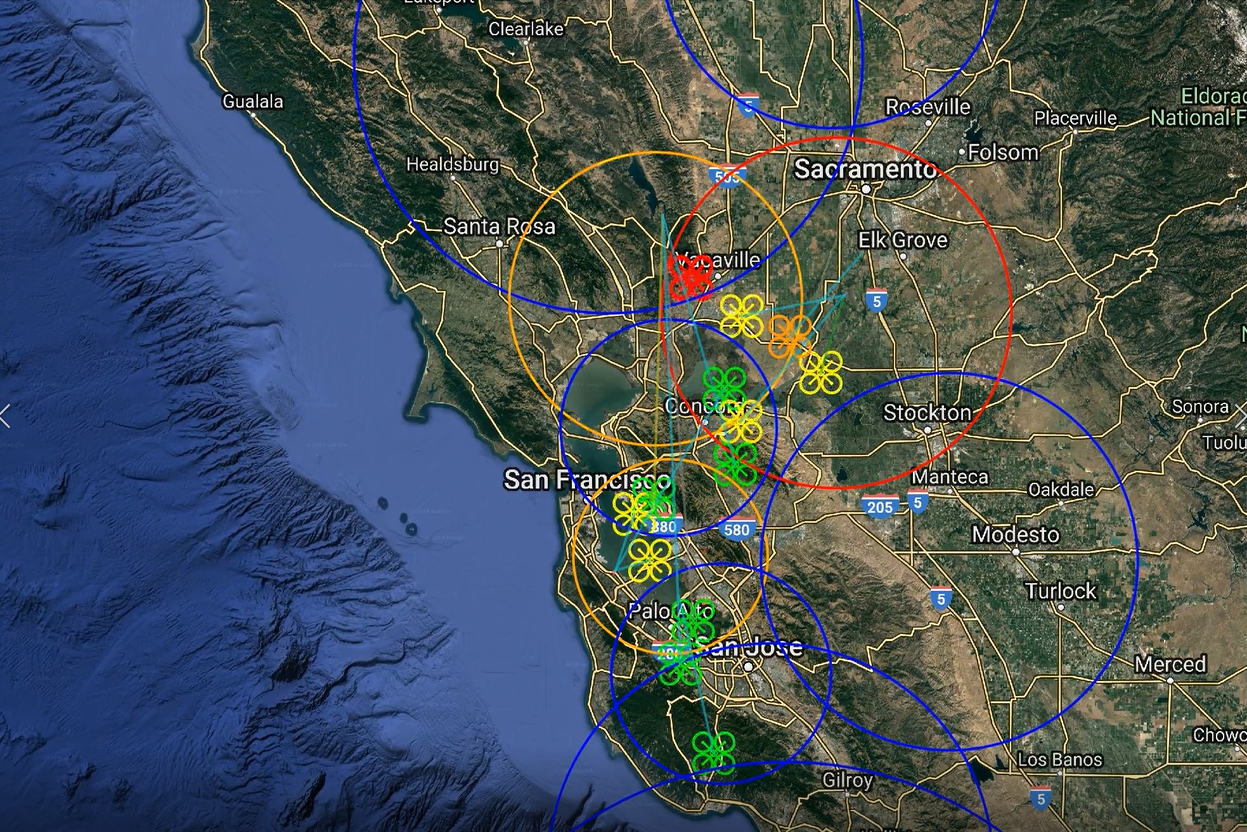
\includegraphics[width=0.75\textwidth]{UAM-TCNS/Towers.PNG}
	\caption[Screenshot of the UAM operations simulation environment ]{Screenshot of the simulation environment - green agents are in flight mode, orange agents are loitering, yellow agents are allocated for landing/passing-through and red agents are those that have landed. If a vertihub controller circle is red, then it will accept no more agents until the agents inside have landed or have been accepted to pass through to another region.
	}
	\label{fig:sim}
\end{figure}

All vertihub controllers must satisfy the following specifications: (1) landing or pass-through requests must be approved in less than $T$ steps and (2) there can be no more than $N$ vehicles in the region of the vertihub. 
All vertiport controllers must satisfy the following condition: no more than $M$ vehicles can land at any given time. The landing time is treated as an environment input and can vary based on the vehicle and weather conditions. The contract between the vertiport and vertihub states that a vertiport may not allow a vehicle to take off for up to $L$ steps and must clear a landing spot in at most $K$ steps. The vertihub controllers have contracts with connected controllers agreeing to let vehicles loiter in their regions for $t < T$ timesteps. These contracts allow vertihub controllers to land or let vehicles pass through while incoming vehicles loiter in neighboring regions.
The resulting video simulations for each setting can be seen in  \href{https://u-t-autonomous.github.io/Decentralized-UAM-Traffic-Management/}{https://u-t-autonomous.github.io/Decentralized-UAM-Traffic-Management/}.
\textcolor{black}{Also included in the link are further comparisons with different physical architectures for vertihub placement -- in particular we compare scenario (i) when the airspace is covered by double the number of the vertihubs. The average loiter time for vehicles in setting (i) was approximately 3\% less per vehicle for the environment with more vertihubs, however, we note that this is not true in general and the average loiter time will depend on the specific network topology and specifications.}
Note that quantitative analysis and optimizing for minimum loiter times are of interest to this problem but the controllers operating in these case studies are only concerned with correctness.

\begin{figure}[h]
\centering
    \subfloat[Landing \label{fig:land}]{
    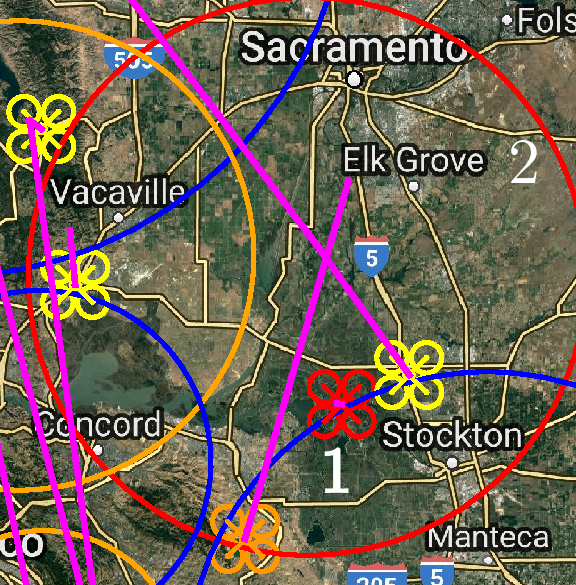
\includegraphics[width=0.32\textwidth]{UAM-TCNS/pics/sequence_100a.png}}~
    \subfloat[Free slot \label{fig:free}]{
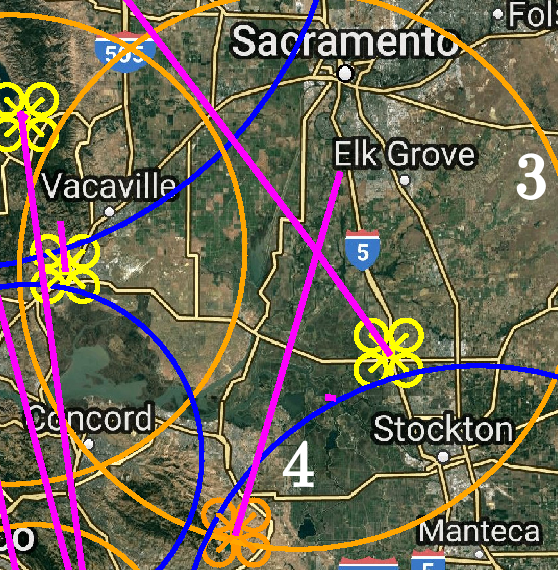
\includegraphics[width=0.32\textwidth]{UAM-TCNS/pics/sequence_103a.png}}~
    \subfloat[Allocated \label{fig:allocate}]{
    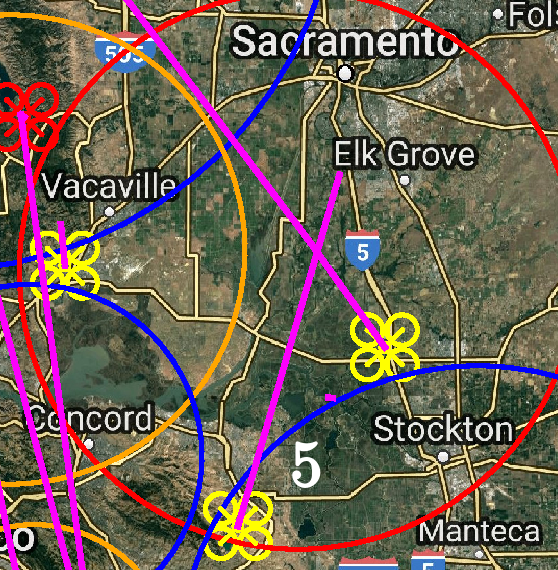
\includegraphics[width=0.32\textwidth]{UAM-TCNS/pics/sequence_104a.png}}
    \caption{\textcolor{black}{Time sequence of a UAV landing ($1$) at a vertiport, which opens up a free slot for the vertihub ($2\rightarrow3$). The hub then allocates another UAV ($4\rightarrow 5$) to land at a free slot in one of the vertiports.}}
    \label{fig:sequence}
\end{figure}

\subsection{Qualitative results}

Figure~\ref{fig:sequence} contains an example of the allocation behavior for multiple agents approaching a single vertihub.
\textcolor{black}{Initially the vertihub is informed by the vertiports that there are no slots available for landing (see $2$ in Fig.~\ref{fig:land}). Subsequent to an agent landing ($1$ lands), an additional slot opens (see $3$ in Fig.~\ref{fig:free}).
Finally, the vertihub allocates a slot to a requesting vehicle ($4$ becomes $5$ in figure~\ref{fig:allocate}).} 

For each simulation setting, the vertihub interactions affect how vehicles are allocated and subsequently where they loiter.
In the case of setting (i), allocation bottlenecks tend to occur upon vehicle launch -- as a vehicle launches it waits for permission to move and thus bottlenecks are limited by the operating number of vehicles in the vertihub.
For setting (ii), there are significantly fewer bottlenecks but they mostly occur as vehicles either enter or exit a region.
For setting (iii) we observe the cascading effect of allocations in each region -- to allocate vehicles in the top region, the vehicles in the middle region must clear and similarly for the middle-lower region interactions.

\subsection{Synthesis time}

We present the synthesis times for the vertihub and vertiport controllers in Table~\ref{tab:hubsyntime}. 
There is an exponential increase in the synthesis time as the number of vertiports in each region is increased.
%Thus, this technique works best when there is not be a large number of vertiports assigned to each vertihub.
The state space of the controllers does not depend on the number of vehicles allowing us to simulate datasets involving large numbers of vehicles. \textcolor{black}{
The centralized synthesis method in~\cite{bh18} could not be run even in the smallest case as the state space is too large. A decentralized, hierarchical procedure is necessary to handle systems of the necessary size and complexity that UAM will require. Other decentralized techniques such as~\cite{bhnfm} can only handle very restrictive classes of specifications and could not be used to generate controllers in this setting.}

We note that since the synthesis for each vertihub is independent of one another once the contracts are generated, the synthesis procedure for the global system is trivially parallelizable. 

\begin{table}[t!]
	\centering
	\caption{Synthesis times for vertihub/vertiport controllers}
	\label{tab:hubsyntime}
	\centering
	\scalebox{0.9}{
		\begin{tabular}{l>{\raggedleft}p{2.5cm}>{\raggedleft}p{2.0cm}>{\raggedleft\arraybackslash}p{1.5cm}}
			\toprule
			& No. of vertiports / No. of landing pads & No. of states in controller ($|Q_i|$) &  Synthesis time (s)  \\
			\midrule
			\multirow{3}*{Vertihub} & 3 & $2.1\times10^4$ & 22.75      \\
			& 4 & $2.7\times10^6$ & 1272.95  \\
			& 5 & $3.4\times10^8$ & 14300.65 \\
			\multicolumn{4}{@{}c@{}}{\makebox[\linewidth]{\dashrule[black]}}\\
			\multirow{3}*{Vertiport}&2 & $6.1\times10^2$ & 0.45      \\
			&4 & $4.3\times10^4$ & 19.12  \\
			&8 & $1.9\times10^8$ & 12403.86 \\
			\bottomrule
	\end{tabular}}
\end{table}

%\section{Conclusion}
\section{Conclusion}
\label{sec_concl}
In this paper, we proposed a general approach to the synthesis of shields for multi-agent systems from temporal logic specifications. Our key contribution is the study of quantitative objectives in the shield synthesis setting. Our work is also the first to consider fairness requirements on the shields. We introduced the notion of interference cost, and discussed several costs and synthesis objectives that are of interest when considering multi-agent systems. We demonstrated the applicability of the proposed approach on a range of quantitative interference requirements by synthesizing shields for a multi-UAV system.

A promising  avenue for future work is to investigate bounded synthesis~\cite{FinkbeinerS13} with quantitative objectives, in order to synthesize distributed shields, which will enhance the efficiency of shields for distributed systems.



